\documentclass[12pt]{report}
\usepackage[parfill]{parskip}
\usepackage[utf8]{inputenc}
\usepackage{graphicx}
\usepackage{amsthm}
\usepackage{amsmath}
\usepackage{amsfonts}
\usepackage{braket}
\usepackage{mathtools}
\usepackage{cancel}
\usepackage[dvipsnames]{xcolor}
\usepackage{hyperref}
\usepackage{todonotes}
\usepackage[capitalize]{cleveref}
\usepackage[section]{placeins}
\usepackage[labelfont=bf]{caption} % bold figure labels
\usepackage[normalem]{ulem} % for strikethrough text
\usepackage[
    % toc,
    % page
    ]{appendix}
\usepackage{tikz}
\usetikzlibrary{decorations.markings,math,calc,braids,intersections,backgrounds}

\creflabelformat{equation}{#2\textup{#1}#3}
\Crefname{equation}{Eqn.}{Eqns.}
\Crefname{figure}{Figure}{Figures}
\newcommand{\crefrangeconjunction}{--}

% \usepackage{commands}

\graphicspath{ {figures/} }
% \FloatBarrier

\title{
{Title}\\
% {\large A Thesis \\presented to \\ the Faculty of California Polytechnic State University, \\San Luis Obispo}\\
}
\author{Max Varverakis}
\date{\today}

\newtheorem{theorem}{Theorem}[chapter]
\newtheorem{corollary}{Corollary}[theorem]
\newtheorem{lemma}[theorem]{Lemma}
\newtheorem{proposition}[theorem]{Proposition}

\theoremstyle{definition}
\newtheorem{definition}{Definition}[chapter]
\newtheorem{example}{Example}[chapter]
% customize end of example symbol
% \AtBeginEnvironment{example}{%
%     \pushQED{\qed}\renewcommand{\qedsymbol}{$\triangle$}%
% }
% \AtEndEnvironment{example}{\popQED\endexample}

% \renewcommand{\bibname}{References}

\includeonly{
    chapters/introduction,
    % chapters/Rep_Theory_Background,
    chapters/Phys_applications,
    % chapters/Top_Background,
    % chapters/The_Braid_Group,
    % chapters/Anyons,
    chapters/Appendix_physics_background,
    % chapters/Appendix_multi_anyon,
    % chapters/tikz_test,
    chapters/TODO,
}

\begin{document}

% load custom commands (placed after begin document so that VSCode intellisence recognizes the commands)
\newcommand{\ehat}{\hat{e}}
\newcommand{\mat}[3]{{{#1}^#2}_#3}
\newcommand{\sotwo}{\textrm{SO}{(2)}}
\newcommand{\C}{\mathbb{C}}
\newcommand{\R}{\mathbb{R}}
\newcommand{\Z}{\mathbb{Z}}
\newcommand{\D}{\mathbb{D}}
\newcommand{\Q}{\mathbb{Q}}
\newcommand{\iv}[1]{{ #1 }^{-1}}
\newcommand{\aut}[1]{\textrm{Aut}\!\left( #1 \right)}
\newcommand{\iso}{\simeq}
\newcommand{\niso}{\not\simeq}
\newcommand{\st}{~\big|~}
\newcommand{\tr}[1]{\textrm{tr}\left(#1\right)}
\newcommand{\size}[1]{\left|#1\right|}
\newcommand{\sheet}[2]{\widetilde{#1}_{#2}}
% \newcommand{\ra}{\right\rangle}
% \newcommand{\la}{\left\langle}
% \newcommand{\lra}[1]{\la{#1}\ra}


% \renewcommand{\vec}[1]{\mathbf{#1}} % Uncomment to use bold vectors
\newcommand{\vd}[1]{\dot{\vec{#1}}}

\maketitle

\tableofcontents
\listoffigures % need short caption for each figure or something like that

\chapter{Introduction}\label{ch:introduction}

The intimate connection between abstract mathematics and the physical world highlights the beautiful complexity of nature. In our efforts to understand the fundamental processes that govern the universe, we grow increasingly reliant on the principles of mathematics. One such tool that bridges the abstract and physical regimes is known as representation theory.

In this thesis, we examine representation theory and observe the physical consequences that emerge from the mathematics. First, we begin in \cref{ch:rep_background} with a brief overview of representation theory. Then in \cref{ch:Phys_applications}, we investigate specific applications of representation theory in the context of quantum physics, arriving at remarkably fundamental results. In \cref{ch:braid_group}, we introduce the braid group and explore some of its representations. Finally, we highlight physical applications of the braid group and its representations in \cref{ch:anyons}.

It is assumed that the reader has a basic understanding of group theory and linear algebra. A familiarity with topology is also required, and the relevant definitions can be found in \cref{ch:top_background}. Notational conventions are chosen to align with the physics literature which at times differs from the standard mathematical notation. Discussions in the later chapters assume a general understanding of classical and quantum mechanics. To those less familiar with those topics and the notation, a supplementary overview is given in \cref{ch:physics_background}.

\chapter{Representation Theory Background}\label{ch:rep_background}

\begin{definition}[Representations of a Group]
    If there is a homomorphism from a group $G$ to a group of operators $U(G)$ on a linear vector space $V$, we say that $U(G)$ forms a \textit{representation} of $G$ with dimension $\dim V$.
\end{definition}

The representation is a map
\begin{equation}
    g\in G\xrightarrow{U} U(g)
\end{equation}
in which $U(g)$ is an operator on the vector space $V$. For a set of basis vectors $\{\hat{e_i},i=1,2,\dots,n\}$, we can realize each operator $U(g)$ as an $n\times n$ matrix $D(g)$.
\begin{equation}
    U(g)\ket{e_i} = \sum_{j=1}^n \ket{e_j}{{D(g)}^j}_i = \ket{e_j}{{D(g)}^j}_i,
\end{equation}
where the first index $j$ is the row index and the second index $i$ is the column index. We use the Einstein summation convention, so repeated indices are summed over. Note that the operator multiplication is defined as
\begin{equation}
    U(g_1)U(g_2) = U(g_1g_2),
\end{equation}
which satisfies the group multiplication rules.

\begin{definition}
    If the homomorphism defining the representation is an isomorphism, then the representation is \textit{faithful}. Otherwise, it is \textit{degenerate}.
\end{definition}

\begin{example}
    Let $G$ be the group of continuous rotations in the $xy$-plane about the origin. We can write $G = \{R(\phi),0\leq\phi\leq2\pi\}$ with group operation $R(\phi_1)R(\phi_2) = R(\phi_1+\phi_2)$. Consider the 2-dimensional Euclidean vector space $V_2$. Then we define a representation of $G$ on $V_2$ by the familiar rotation operation
    \begin{align}
        \hat{e}_1' &= U(\phi)\hat{e}_1 = \hat{e}_1\cdot\cos\phi + \hat{e}_2\cdot\sin\phi\\
        \hat{e}_2' &= U(\phi)\hat{e}_2 = -\hat{e}_1\cdot\sin\phi + \hat{e}_2\cdot\cos\phi.
    \end{align}
This gives us the matrix representation
\begin{equation}
    D(\phi) = \begin{pmatrix}
        \cos\phi & -\sin\phi\\
        \sin\phi & \cos\phi
    \end{pmatrix}.
\end{equation}
To further illustrate this representation, if we consider an arbitrary vector $\hat{e_i}x^i=\vec{x}\in V_2$, then we have
\begin{equation}
    \vec{x}' = U(\phi)\vec{x} = \hat{e}_j{x'}^j,
\end{equation}
where ${x'}^j = {{D(\phi)}^j}_i x^i$.
\end{example}

\begin{definition}[Equivalence of Representations]
    For a group $G$, two representations are \textit{equivalent} if they are related by a similarity transformation. Equivalent representations form an equivalence class.
\end{definition}

To determine whether two representations belong to the same equivalence class, we define
\begin{definition}[Characters of a Representation]
    The \textit{character} $\chi(g)$ of an element $g\in G$ in a representation $U(g)$ is defined as $\chi(g) = \text{Tr}~D(g)$.
\end{definition}
Since trace is independent of basis, the character serves as a class label.

Vector space representations of a group have familiar substructures, which are useful in constructing representations of the group.
\begin{definition}[Invariant Subspace]
    Let $U(G)$ be a representation of $G$ on a vector space $V$, and $W$ a subspace of $V$ such that $U(g)\ket{x}\in W$ for all $\vec{x}\in W$ and $g\in G$. Then $W$ is an \textit{invariant subspace} of $V$ with respect to $U(G)$. An invariant subspace is \textit{minimal} or \textit{proper} if it does not contain any non-trivial invariant subspace with respect to $U(G)$.
\end{definition}

The identification of invariant subspaces on vector space representations leads to the following distinction of the representations.
\begin{definition}[Irreducible Representation]
    A representation $U(G)$ on $V$ is \textit{irreducible} if there is no non-trivial invariant subspace in $V$ with respect to $U(G)$. Otherwise, it is \textit{reducible}. If $U(G)$ is reducible and its orthogonal complement to the invariant subspace is also invariant with respect to $U(G)$, then the representation is \textit{fully reducible}.
\end{definition}

\begin{example}
    Under the group of 2-dimensional rotations, consider the 1-dimensional subspace spanned by $\ehat_1$. This subspace is not invariant under 2-dimensional rotations, because a rotation of $\ehat_1$ by $\pi/2$ results in the vector $\ehat_2$ that is clearly not in the subspace spanned by $\ehat_1$. A similar argument shows that the subspace spanned by $\ehat_2$ is not invariant under 2-dimensional rotations.

    However, consider the linear combination of basis vectors
    \begin{equation}
        \ehat_\pm = \frac{1}{\sqrt{2}}\left( \mp\ehat_1 + i\ehat_2 \right),
    \end{equation}
    where $i = \sqrt{-1}$. Then a rotation by angle $\phi$, denoted in operator form as $U(\phi)$, acts on $\ehat_\pm$ by
    \begin{align}
        U(\phi)\ket{\ehat_+} &= U(\phi)\frac{1}{\sqrt{2}}(-\ehat_1 + i\ehat_2) \\
        &= \frac{1}{\sqrt{2}}(-U(\phi)\ket{\ehat_1} + iU(\phi)\ket{\ehat_2}) \nonumber \\
        &= \frac{1}{\sqrt{2}}\left( -\ehat_1\cos\phi - \ehat_2\sin\phi -i\ehat_1\sin\phi + i\ehat_2\cos\phi \right) \nonumber \\
        &= \frac{1}{\sqrt{2}}\left( -\ehat_1(\cos\phi+ i\sin\phi) +i\ehat_2(\cos\phi-i\sin\phi) \right) \nonumber \\
        % &= \frac{1}{\sqrt{2}}\big(\ehat_1(-\cos\phi+i\sin\phi) + \ehat_2(i\cos\phi + \sin\phi)\big) \nonumber \\
        % &= \frac{1}{\sqrt{2}}(-\ehat_1 + i\ehat_2)(\cos\phi - i\sin\phi) \nonumber \\
        & \colorbox{red}{\textbf{Not Done}} \nonumber \\
        &= \ehat_+ (\cos\phi - i\sin\phi) \nonumber \\
        &= \ehat_+ e^{-i\phi}, \\
        \textrm{and } U(\phi)\ket{\ehat_-} &= \ehat_- e^{i\phi}.
    \end{align}

\end{example}



The irreducible representation matrices satisfy \colorbox{red}{orthonormality and completeness} relations.\textbf{ Thm. 3.5}?

\begin{example}[Generator of $\sotwo$]
    Consider the rotations of a 2-dimensional Euclidean vector space about the origin. Let $\ehat_1$ and $\ehat_2$ be orthonormal basis vectors of this space. Using geometry, we can determine how a rotation by some angle $\phi$, written in operator form as $R(\phi)$, acts on the basis vectors:
    \begin{align}
        R(\phi)\ehat_1 &= \ehat_1\cos\phi + \ehat_2\sin\phi \label{eq:rot_1}\\
        R(\phi)\ehat_2 &= -\ehat_1\sin\phi + \ehat_2\cos\phi.\label{eq:rot_2}
    \end{align}
    In matrix form, we can write
    \begin{equation}
        R(\phi) = 
        \begin{pmatrix}
            \cos\phi & -\sin\phi \\
            \sin\phi & \cos\phi
        \end{pmatrix}
    \end{equation}
    which allows us to write \cref{eq:rot_1,eq:rot_2} in a condensed form
    \begin{equation}
        R(\phi)\ehat_i = \ehat_j{{R(\phi)}^j}_i,
    \end{equation}
    where we are summing over $j=1,2$.

    Now, let $\vec{x}$ be an arbitrary vector in the plane. Then $\vec{x}$ has components $x^i$ in the basis $\{\ehat_i\}$, where $i=1,2$. Equivalently, we can write $\vec{x}=\ehat_i x^i$. Then under rotations, $\vec{x}$ transforms in accordance to the basis vectors
    \begin{align}
        R(\phi)\vec{x} &= R(\phi)\ehat_i x^i \label{eq:rot_vec} \\
        &= \ehat_j{{R(\phi)}^j}_i x^i \nonumber \\
        &= \left( \ehat_1\mat{R(\phi)}{1}{i} + \ehat_2\mat{R(\phi)}{2}{i} \right)x^i \nonumber \\
        &= \left( \ehat_1\cos\phi + \ehat_2\sin\phi \right) x^1 + \left( \ehat_1(-\sin\phi) + \ehat_2\cos\phi \right) x^2 \nonumber \\
        &= \left( x^1\cos\phi - x^2\sin\phi \right)\ehat_1 + \left( x^1\sin\phi + x^2\cos\phi \right)\ehat_2.  \nonumber
    \end{align}

    Observe that $R(\phi)R^\top(\phi) = E$ where $E$ is the identity matrix. This is precisely what defines \textit{orthogonal matrices}. For 2-dimensional vectors in the plane, it is clear that these rotations do not change the length of said vectors. This can be verified by using \cref{eq:rot_vec}:
    \begin{align}
        |R(\phi)\vec{x}|^2 &= |\ehat_j\mat{R(\phi)}{j}{i} x^i|^2 \\
        &= \left|\left( x^1\cos\phi - x^2\sin\phi \right)\ehat_1 + \left( x^1\sin\phi + x^2\cos\phi \right)\ehat_2\right|^2 \nonumber \\
        &= {\left( x^1\cos\phi - x^2\sin\phi \right)}^2 + {\left( x^1\sin\phi + x^2\cos\phi \right)}^2 \nonumber \\
        &= \left( \cos^2\phi + \sin^2\phi \right)x^1 x_1 + \left( \sin^2\phi + \cos^2\phi \right)x^2 x_2 \nonumber \\
        &= x^1 x_1 + x^2 x_2 = |\vec{x}|^2. \nonumber
    \end{align}

    Similarly, notice that for any continuous rotation by angle $\phi$, $\det R(\phi) = \cos^2\phi+\sin^2\phi = 1$. In general, orthogonal matrices have determinant equal to $\pm1$. However, the result of the above determinant of $R(\phi)$ implies that all continuous rotations in the 2-dimensional plane have determinant equal to $+1$. These are the \textit{special orthogonal matrices of rank 2}. This family of matrices is denoted $\sotwo$. Furthermore, there is a one-to-one correspondence with $\sotwo$ matrices and rotations in a plane.

    We define the group of continuous rotations in a plane by letting $R(0) = E$ be the identity element corresponding to no rotation (i.e., a rotation by angle $\phi=0$), and defining the inverse of a rotation as $R^{-1}(\phi) = R(-\phi) = R(2\pi-\phi)$. This group can be called the $\sotwo$ group. Lastly, we define group multiplication as $R(\phi_1)R(\phi_2) = R(\phi_1+\phi_2)$ and note that $R(\phi) = R(\phi\pm2\pi)$, which can be verified geometrically. Thus, group elements of $\sotwo$ can be labelled by the angle of rotation $\phi\in[0,2\pi)$.

    Now we can find a generator of $sotwo$ by considering an infinitesimal rotation, labelled by some infinitesimal angle $d\phi$. Then this is equivalent to the identity plus some small rotation, which we can write as
    \begin{equation}
        R(\textrm{d}\phi) = E - i \textrm{d}\phi J
    \end{equation}
    where the scalar quantity $-i$ is introduced for later convenience and $J$ is some quantity independent of the rotation angle. If we consider the rotation $R(\phi + \textrm{d}\phi)$, then there are two equivalent ways to interpret this rotation
    \begin{align}
        R(\phi + \textrm{d}\phi) &= R(\phi)R(\textrm{d}\phi) = R(\phi)(E - i \textrm{d}\phi J) = R(\phi) - i \textrm{d}\phi R(\phi)J \\
        R(\phi + \textrm{d}\phi) &= R(\phi) + \textrm{d}R(\phi) = R(\phi) + \textrm{d}\phi\frac{\textrm{d}R(\phi)}{\textrm{d}\phi}
    \end{align}
    where the second equation can be thought of as a Taylor expansion of $R(\phi + \textrm{d}\phi)$ about $\phi$. Equating the two expressions for $R(\phi + \textrm{d}\phi)$ yields
    \begin{equation}
        \textrm{d}R(\phi) = -i\textrm{d}\phi R(\phi)J.
    \end{equation}
    Solving this differential equation (with boundary condition $R(0)=E$) provides us with an equation for any group element involving $J$:
    \begin{equation}
        R(\phi) = e^{-i\phi J},
    \end{equation}
    where $J$ is called the \textit{generator} of the group.
\end{example}

\chapter{Examples in Physics}\label{ch:Phys_applications}

The goal of this chapter is to highlight some key results in physics through the lens of representation theory. The intimate connection between quantum mechanics and the representations discussed below offers a unique perspective on the emergence of the fundamental properties of quantum physics. To best illustrate the application of representation theory in quantum mechanics, notation is chosen to agree with the physics conventions. For those not as familiar with Dirac notation and the related quantum mechanical concepts, please refer to \cref{ch:physics_background}.

\section{Rotations in a plane and the group SO(2)}\label{sec:SO2}

% \textcolor{blue}{Intro paragraph here?}

\subsection{The rotation group}
Consider the rotations of a 2-dimensional Euclidean vector space about the origin. Let $\e_1$ and $\e_2$ be orthonormal basis vectors of this space. Using geometry, we can determine how a rotation by some angle $\phi$, written in operator form as $R(\phi)$, acts on the basis vectors:
\begin{align}
    R(\phi)\e_1 &= \e_1\cos\phi + \e_2\sin\phi \label{eq:rot_1}\\
    R(\phi)\e_2 &= -\e_1\sin\phi + \e_2\cos\phi.\label{eq:rot_2}
\end{align}
In matrix form, we can write
\begin{equation}
    R(\phi) = 
    \begin{bmatrix}
        \cos\phi & -\sin\phi \\
        \sin\phi & \cos\phi
    \end{bmatrix}
\end{equation}
which allows us to write \cref{eq:rot_1,eq:rot_2} in a condensed form
\begin{equation}
    R(\phi)\e_i = {{R(\phi)}^j}_i\e_j,
\end{equation}
with an implicit sum over the repeated index $j=1,2$.
% The set of these rotation matrices forms a degree 2 representation of the rotation group.

Let $\vec{x}$ be an arbitrary vector in the plane. Then $\vec{x}$ has components $x_i$ in the basis $\{\e_i\}$, where $i=1,2$. Equivalently, we can write $\vec{x}=\e_i x_i$, where again we implicitly sum over repeated indices. Then $\vec{x}$ transforms under rotations in accordance to the basis vectors
\begin{align}
    R(\phi)\vec{x} &= R(\phi)\e_i x_i \nonumber \\
    &= {{R(\phi)}^j}_i x_i \e_j \nonumber \\
    &= \left( \mat{R(\phi)}{j}{1}x_1 + \mat{R(\phi)}{j}{2}x_2 \right) \e_j \nonumber \\
    % &= \left( \e_1\mat{R(\phi)}{1}{i} + \e_2\mat{R(\phi)}{2}{i} \right)x_i \nonumber \\
    % &= \left( \e_1\cos\phi + \e_2\sin\phi \right) x_1 + \left( \e_1(-\sin\phi) + \e_2\cos\phi \right) x_2 \nonumber \\
    &= \left( x_1\cos\phi - x_2\sin\phi \right)\e_1 + \left( x_1\sin\phi + x_2\cos\phi \right)\e_2. \label{eq:rot_vec} 
\end{align}

Notice that $R(\phi)R^\top(\phi) = I$ where $I$ is the identity matrix. This is precisely what defines \textit{orthogonal matrices}. For 2-dimensional vectors in the plane, it is clear that these rotations do not change the length of said vectors. This can be verified by using \cref{eq:rot_vec}:
\begin{align*}
    |R(\phi)\vec{x}|^2 &= |\mat{R(\phi)}{j}{i} x_i\e_j|^2 \\
    &= \left|\left( x_1\cos\phi - x_2\sin\phi \right)\e_1 + \left( x_1\sin\phi + x_2\cos\phi \right)\e_2\right|^2 \\
    &= {\left( x_1\cos\phi - x_2\sin\phi \right)}^2 + {\left( x_1\sin\phi + x_2\cos\phi \right)}^2 \\
    &= \left( \cos^2\phi + \sin^2\phi \right)x_1^2 + \left( \sin^2\phi + \cos^2\phi \right)x_2^2 \\
    &= x_1^2 + x_2^2 = |\vec{x}|^2.
\end{align*}

Similarly, notice that for any continuous rotation by angle $\phi$, $\det R(\phi) = \cos^2\phi+\sin^2\phi = 1$. In general, orthogonal matrices have determinant equal to $\pm1$. However, the result of the above determinant of $R(\phi)$ implies that all continuous rotations in the 2-dimensional plane have determinant equal to $+1$. These are the \textit{special orthogonal matrices of rank 2}. This family of matrices is denoted SO(2). Furthermore, there is a one-to-one correspondence with SO(2) matrices and rotations in a plane.

We define the group of continuous rotations in a plane by letting $R(0) = I$ be the identity element corresponding to no rotation (i.e., a rotation by angle $\phi=0$), and defining the inverse of a rotation as $R^{-1}(\phi) = R(-\phi) = R(2\pi-\phi)$. Lastly, we define group multiplication as $R(\phi_1)R(\phi_2) = R(\phi_1+\phi_2)$ and note that $R(\phi) = R(\phi\pm2\pi)$, which can be verified geometrically. Although SO(2) is technically a 2-dimensional representation of a more abstract rotation group, it is often referred to as the rotation group due to the nature of the construction. Thus, group elements of SO(2) can be labelled by the angle of rotation $\phi\in[0,2\pi)$.

\subsection{Infinitesimal rotations}\label{sub:inf_rot}
% Now we can find a generator of SO(2) by considering
Consider an infinitesimal rotation labelled by some infinitesimal angle $d\phi$. This is equivalent to the identity plus some small rotation, which can be written as
\begin{equation}
    R(d\phi) = I - i d\phi J \label{eq:dphi}
\end{equation}
where the scalar quantity $-i$ is introduced for later convenience and $J$ is some quantity independent of the rotation angle. If we consider the rotation $R(\phi + d\phi)$, then there are two equivalent ways to interpret this rotation. Namely,
\begin{align}
    R(\phi + d\phi) &= R(\phi)R(d\phi) = R(\phi)(I - i d\phi J) = R(\phi) - i d\phi R(\phi)J,\label{eq:dphi1} \\
    R(\phi + d\phi) &= R(\phi) + d\phi\frac{dR(\phi)}{d\phi},\label{eq:dphi2}
    % R(\phi) + dR(\phi) =
\end{align}
where the \cref{eq:dphi2} can be thought of as a Taylor expansion of $R(\phi + d\phi)$ about $\phi$. Equating the two expressions for $R(\phi + d\phi)$ yields
\begin{equation}
    dR(\phi) = -id\phi R(\phi)J.
\end{equation}
Solving this differential equation (with boundary condition $R(0)=I$) provides us with an equation for any group element involving $J$:
\begin{equation}
    R(\phi) = e^{-i\phi J},
\end{equation}
where $J$ is called the \textit{generator} of the group.

The explicit form of $J$ is found as follows. To first order in $d\phi$, we have
\begin{align*}
    R(d\phi) &= \begin{bmatrix}
        1 & -d\phi \\
        d\phi & 1
    \end{bmatrix}.
\end{align*}
Comparing to \cref{eq:dphi},
\begin{align*}
    I - i d\phi J &= \begin{bmatrix}
        1 & -d\phi \\
        d\phi & 1
    \end{bmatrix} \implies J = \begin{bmatrix}
        0 & -i \\
        i & 0
    \end{bmatrix}.
\end{align*}

Notice that $J^2 = I$, which implies that even powers of $J$ equal the identity matrix and odd powers of $J$ equal $J$. Taylor expanding $e^{-iJ\phi }$ gives
\begin{align*}
    R(\phi) = e^{-iJ\phi} &= I - iJ\phi - I \frac{\phi^2}{2!} + iJ\frac{\phi^3}{3!} + \cdots \\
    &= I\left( \sum_{n=0}^{\infty} {(-1)}^n \frac{\phi^{2n}}{(2n)!} \right) - iJ\left( \sum_{n=0}^{\infty} {(-1)}^n \frac{\phi^{2n+1}}{(2n+1)!} \right) \\
    &= I\cos\phi - iJ\sin\phi \\
    &= \begin{bmatrix}
        \cos\phi & -\sin\phi \\
        \sin\phi & \cos\phi
    \end{bmatrix}.
\end{align*}
Therefore, the generator $J$ can be used to recover the rotation matrix for an arbitrary angle $\phi$.
% Moreover, the corresponding map $R(\phi)\mapsto e^{iJ\phi}$ is a valid homomorphism that respects the periodic nature of SO(2).

\subsection{Irreducible representations of SO(2)}\label{sub:irr_so2}

Equipped with the generator $J$, we can construct the irreducible representations of SO(2). First, consider a representation $U$ of SO(2) defined on a finite dimensional vector space $V$. Then $U(\phi)$ is the corresponding representation of $R(\phi)$. The same argument as in \cref{sub:inf_rot} can be applied to an infinitesimal rotation to give
\begin{align*}
    U(\phi) = e^{-iJ\phi},
\end{align*}
which is an operator on $V$ (for convenience, the same symbol $J$ is used to denote the generator of the representation).
% As seen in \cref{sub:inf_rot}, a one-dimensional representation of SO(2) is given by $R(\phi)\mapsto e^{-iJ\phi}$, where $J$ is the generator of the group. This representation is clearly irreducible, as there are no non-trivial invariant subspaces of a one-dimensional vector space.

Since $U$ is a representation of rotations, it preserves the length of vectors for all angles $\phi$. Thus, for all vectors $\vec{a}$ (alternatively expressed as $\ket{a}$) in $V$ and $\phi\in[0,2\pi)$, we have
\begin{align*}
    \size{\vec{a}}^2 = \size{U(\phi)\vec{a}}^2
    &\iff \braket{a|a} = \braket{U(\phi)a|U(\phi)a} = \braket{a|{U(\phi)}^\dagger U(\phi)|a} \\
    &\iff U(\phi)^\dagger U(\phi) = I \\
    &\iff e^{iJ^\dagger\phi}e^{-iJ\phi} = e^{-i(J-J^\dagger)\phi} = 1 \\
    &\iff J = J^\dagger,
\end{align*}
where $\dagger$ is the conjugate transpose. Additionally, \textit{Dirac notation} is adopted for the above calculations. More information about Dirac notation can be found in \cref{ch:physics_background}. As a result of this calculation, not only must $U$ be unitary, but the generator $J$ must be Hermitian. In particular, we will be leveraging the fact that Hermitian operators have real eigenvalues. This fact becomes especially important in the physical interpretation of the representations of 3-dimensional rotations in \cref{sec:phys_SO3}

According to \cref{cor:abelian_irred}, the abelian nature of SO(2) implies that all of its irreducible representations are one-dimensional. Then for any $\ket{\alpha}\in V$, the minimal subspace containing $\ket{\alpha}$ that is invariant under SO(2) is one-dimensional. Hence,
\begin{align*}
    J\ket{\alpha} &= \alpha\ket{\alpha}, \\
    U(\phi)\ket{\alpha} &= e^{-iJ\phi}\ket{\alpha} = e^{-i\alpha\phi}\ket{\alpha},
\end{align*}
where the (real) number $\alpha$ is used as a label for the eigenvector of $J$ with eigenvalue $\alpha$. The periodicity conditions of SO(2) imply that $\ket{\alpha} = U(2\pi)\ket{\alpha}$, or equivalently, $e^{-i2\pi\alpha} = 1$. This implies that $\alpha$ must be an integer, as $e^{-i2\pi m} = 1$ for $m\in\mathbb{Z}$. Then $U$ has a corresponding 1-dimensional representation for an integer $m$, defined by
\begin{align*}
    J\ket{m} = m\ket{m}, \\
    U^m(\phi)\ket{m} = e^{-im\phi}\ket{m}.
\end{align*}
Though already true by \cref{cor:abelian_irred}, these representations are clearly irreducible, as there is no way to reduce the dimension of a 1-dimensional representation.

In general, the \textit{single-valued irreducible representations of SO(2)} are defined as
\begin{equation}
    U^m(\phi) = e^{-im\phi},
\end{equation}
for $m\in\Z$.

If $m=0$, then $R(\phi)\mapsto U^0(\phi) = 1$, which corresponds to the trivial representation. If instead $m=1$, then $R(\phi)\mapsto U^1(\phi) = e^{-i\phi}$, which maps rotations in SO(2) to distinct points on the unit circle in the complex plane. The $m=1$ representation is faithful because each rotation by $\phi$ has a unique image under $U^1(\phi)$, which is clear when interpreting rotations of unit vectors geometrically. As $\phi$ ranges from 0 to $2\pi$, $U^1$ traces over the unit circle in $\C$ in the clockwise direction. Similarly, $U^{-1}$ traces over the unit circle in the counterclockwise direction because $U^{-1}(\phi)=e^{i\phi}$. The $m=-1$ case is therefore faithful as well. In general, $U^n$ covers the unit circle $\size{n}$ times as $\phi$ ranges from 0 to $2\pi$, and is not faithful for $n\neq\pm1$.

The irreducible representations of SO(2) are orthonormal in the sense that
\begin{align}
    \frac{1}{2\pi}\int_{0}^{2\pi}{\bigl(U^m(\phi)\bigr)}^\dagger U^n(\phi) \,d\phi = \frac{1}{2\pi}\int_{0}^{2\pi} e^{-i(n-m)\phi} \,d\phi = \delta_{nm},\label{eq:orthogonality}
\end{align}
where $\delta_{nm}$ is the Kronecker delta.
Moreover, the irreducible representations satisfy the completeness relation:
\begin{align}
    \begin{split}    
    \sum_{m\in\Z} U^m(\phi){(U^m(\phi'))}^\dagger 
        &= \sum_{m=-\infty}^\infty e^{-im(\phi-\phi')} \\
        &= 1 + 2\sum_{m=1}^{\infty}\cos(m(\phi-\phi')) \\
        &= 2\pi\delta(\phi-\phi'),
    \end{split}\label{eq:completeness}
\end{align}
where the last equality comes from the fact that the Fourier series of the Dirac delta is a sum over all frequencies of cosines (since it is an even distribution). The completeness relation implies that any appropriately defined function can be expressed in terms of the irreducible representations of SO(2), by integrating over $\phi$. This is analogous to a Fourier series expansion.
% For example, for a function $f(\phi)$, we have
% \begin{align*}
%     f(\phi) = \sum_{m=-\infty}^{\infty}\left( \frac{1}{2\pi}\int_{0}^{2\pi} f(\phi)e^{-im\phi}\,d\phi \right)e^{im\phi}
% \end{align*}
These relations will be exploited in \cref{sub:SO2_decomp}.
% \begin{align*}
%     \sum_{n}\frac{1}{2\pi}\int_{-\infty}^{\infty} e^{-in(\phi-\phi')} f(\phi) \,d\phi
% \end{align*}
% Since SO(2) is a continuous group where the group elements are labelled by the continuous parameter $\phi$, we must integrate over all possible values of $\phi$ to obtain such relations. 

\subsection{Multivalued representations}\label{sub:multi_so2}
If we relax the periodic condition on $U$ to $U(2n\pi) = I$ for some $n\in\Z$, then the resulting 1-dimensional irreducible representations of SO(2) become multivalued. Consider the same construction of $U^m$ in \cref{sub:irr_so2}, but now with $m\in\Q$. For $m=\frac{1}{2}$, we have
\begin{align*}
    U^{1/2}(2\pi + \phi) &= e^{-i\pi - i\frac{\phi}{2}} = -e^{-i\frac{\phi}{2}} = -U^{1/2}(\phi).
\end{align*}
Hence, the rotation $R(\phi)$ is assigned to both $\pm e^{-i\frac{\phi}{2}}$ in the $U^{1/2}$ representation. For this reason, it can be said that $U^{1/2}$ is a \textit{two-valued} representation of SO(2).

Despite this ambiguity in the realization of rotations in SO(2), the modified periodicity condition is still satisfied, as $U^{1/2}(4\pi) = e^{-i2\pi} = 1$. In other words, the double-valued representation of SO(2) traverses the unit circle twice before returning to the identity. In general, $U^{n/m}$ is an $m$-valued representation of SO(2) for $\frac{n}{m}\in\Q$ and $\gcd(n,m)=1$.

The physical importance of these irreducible representations will be discussed when generalizing to rotations in 3-dimensional space in \cref{sec:phys_SO3}.

\subsection{State vector decomposition}\label{sub:SO2_decomp}
The concept of $J$ generating 2-dimensional rotations is summarized in the following example. Consider a particle in a plane with polar coordinates $(r,\phi)$. The state vector of this particle is $\ket{\phi}$, where the coordinate $r$ is suppressed in the vector notation, as the action of SO(2) preserves vector lengths. Note that the state vector $\ket{\phi}$ belongs to some Hilbert space $V$ that is not necessarily the same as the physical space of the particle.

In this angle-basis, we have $U(\theta)\ket{\phi} = \ket{\theta+\phi}$. Then $\ket{\phi}$ can be decomposed as
\begin{align*}
    \ket{\phi} = U(\phi)\ket{\mathcal{O}} = e^{-iJ\phi}\ket{\mathcal{O}},
\end{align*}
where $\ket{\mathcal{O}}$ is a ``standard'' state vector aligned with a pre-selected axis. The triviality of this result must not be overlooked, for it is important to note that any arbitrary state vector $\ket{\phi'}$ can be decomposed into $e^{-iJ\phi'}$ acting on $\ket{\mathcal{O}}$~\cite{Tung1985}. This notion generalizes beyond the 2-dimensional case, and will be revisited for rotations in 3 spatial dimensions in \cref{sec:SO3}.

The orthogonality and completeness relations given in \cref{eq:orthogonality,eq:completeness} imply that
% \begin{align*}
%     \sum_{m} \ket{m}\bra{m} = I.
% \end{align*}
% Thus, 
the state $\ket{\phi}$ can be decomposed into a linear combination of the eigenvectors of $J$:
\begin{align*}
    \ket{\phi} = \left( \sum_{m} \ket{m}\bra{m} \right)\ket{\phi} = \sum_{m} \braket{m|\phi}\ket{m},
\end{align*}
where
\begin{align*}
    \braket{m|\phi} = \braket{m|U(\phi)|\mathcal{O}} = \braket{U^\dagger(\phi)m|\mathcal{O}} = \braket{e^{im\phi}m|\mathcal{O}} = e^{-im\phi}\braket{m|\mathcal{O}}
\end{align*}
is the projection of $\ket{\phi}$ onto the eigenvector $\ket{m}$ of $J$. 
% Note that $m$ is left unspecified, as the allowable values of $m$ depend on the representation of SO(2) and thus the vector space $V$.

By construction, the eigenstates of $J$ are invariant under rotations, so we are free to modify them up to a phase factor (i.e., pick  different representatives from the eigenspaces). For example, we can choose the basis vector $\ket{m}$ to instead be $e^{i\phi_0 m}\ket{m}$ for some $\phi_0\in[0,2\pi)$.  With this in mind, all eigenvectors $\ket{m}$ can be oriented along the direction of $\ket{\mathcal{O}}$ so that $\braket{m|\mathcal{O}} = 1$. Again, note that the inner product $\braket{m|\mathcal{O}}$ is a projection of the \textit{state} $\ket{m}$ onto the \textit{state} $\ket{\mathcal{O}}$, not to be confused with the projection of position vectors in the physical space of this system.

Thus, we can write the state vector $\ket{\phi}$ as
\begin{align}
    \ket{\phi} = \sum_{m} e^{-im\phi}\ket{m}.\label{eq:phi2m}
\end{align}
As a result, the action of $J$ on the state $\ket{\phi}$ can be written as
\begin{align*}
    J\ket{\phi} = \sum_{m} e^{-im\phi} J\ket{m} = \sum_{m} m e^{-im\phi}\ket{m} = \sum_{m} i \frac{\partial}{\partial\phi} \left( e^{-im\phi}\ket{m} \right) = i\frac{\partial}{\partial\phi}\ket{\phi}.
\end{align*}

For fixed $m$, multiplying \cref{eq:phi2m} by $\frac{1}{2\pi} e^{im\phi}$ and integrating over $\phi$, we obtain
\begin{align*}
    \frac{1}{2\pi}\int_{0}^{2\pi} e^{im\phi}\ket{\phi} \,d\phi 
        &= \sum_n \left( \frac{1}{2\pi}\int_{0}^{2\pi}e^{-i(n-m)\phi}\,d\phi \right)\ket{n} \\
        &= \sum_n \left( \frac{1}{2\pi}\int_{0}^{2\pi}{(U^m(\phi))}^\dagger U^n(\phi)\,d\phi \right)\ket{n} \\
        &= \sum_n \delta_{nm}\ket{n} = \ket{m}.
\end{align*}

Then for an arbitrary state $\ket{\psi}\in V$, it follows that
\begin{align*}
    \ket{\psi} = \sum_m \braket{m|\psi}\ket{m} 
        &= \frac{1}{2\pi}\int_{0}^{2\pi} \left( \sum_m e^{im\phi}\braket{m|\psi} \right)\ket{\phi} \,d\phi \\
        &= \frac{1}{2\pi}\int_{0}^{2\pi} \left( \sum_m \braket{\phi|m}\braket{m|\psi} \right)\ket{\phi} \,d\phi \\
        &= \frac{1}{2\pi}\int_{0}^{2\pi} \bra{\phi}\Biggl( \underbrace{\sum_m \ket{m}\bra{m}}_{\textrm{identity}} \Biggr)\ket{\psi}\ket{\phi} \,d\phi \\
        &= \frac{1}{2\pi}\int_{0}^{2\pi} \braket{\phi|\psi}\ket{\phi} \,d\phi \\
        &= \frac{1}{2\pi}\int_{0}^{2\pi} \psi(\phi)\ket{\phi} \,d\phi,
\end{align*}
where $\braket{\phi|\psi}$ is written as the \textit{wavefunction} $\psi(\phi)$ since $\phi$ is a continuous parameter.
% \begin{align*}
%     \psi(\phi) = \braket{\phi|\psi} = \frac{1}{2\pi}\int_{0}^{2\pi} e^{im\phi}\ket{\phi} \,d\phi
% \end{align*}

% \textcolor{red}{Add wavefunction description for uncountably infinite-dim Hilbert space. How you can write $\braket{x|\Psi}$ as just the \textit{wavefunction} $\Psi(x)$ since $x$ is a continuous variable.}

Then the action of $J$ in the $\phi$-basis generalizes to
\begin{align*}
    \braket{\phi|J|\psi} = \braket{J^\dagger \phi|\psi} = -i\frac{\partial}{\partial\phi}\braket{\phi|\psi} = -i\frac{\partial}{\partial\phi}\psi(\phi).
\end{align*}
% where we have projected $J\ket{\psi}$ onto the $\phi$-basis. 
If we let $x$ and $y$ be the Cartesian coordinates of the plane, then
\begin{align*}
    \phi = \arctan\left(\frac{y}{x}\right) \implies \frac{\partial}{\partial\phi} 
        &= \frac{\partial x}{\partial \phi}\frac{\partial}{\partial x} + \frac{\partial y}{\partial \phi}\frac{\partial}{\partial y} \\
        &= \frac{\partial}{\partial\phi}\left( r\cos\phi \right)\frac{\partial}{\partial x} + \frac{\partial}{\partial\phi}\left( r\sin\phi \right)\frac{\partial}{\partial y} \\
        &= -y\frac{\partial}{\partial x} + x\frac{\partial}{\partial y} \\
        &= (\vec{r}\times\vec{\nabla})\cdot\e_z,
\end{align*}
where $\vec{r} = {[x,y,z]}^\top$ and $\vec{\nabla} = {\left[\frac{\partial}{\partial x},\frac{\partial}{\partial y},\frac{\partial}{\partial z}\right]}^\top$. Therefore, the general form of $J$ is
\begin{align}\label{eq:SO2_J}
    J = -i \frac{\partial}{\partial\phi} = -i \left( \vec{r}\times\vec{\nabla} \right)\cdot\e_z.
\end{align}
This result is of particular significance to quantum mechanics, as $J$ has the same form as the orbital \textit{angular momentum operator} $\hat{L}_z$ (normalized to $\hbar$ here), where $z$ is the axis of rotation of the plane\cite{Hall2013,Griffiths2018}.

% Next, a similar construction will be done for the group of continuous translations in one dimension.

\section{Continuous 1-dimensional translations}
% \begin{itemize}
%     % \item Look at the translation group $\R^n$ and its Lie algebra $\mathfrak{t}(n)$.
%     \item Look at the 1D translation group $T$ and its Lie algebra $\mathfrak{t}(1)$.
%     \item Go through same process as SO(2) for $T$ in terms of infinitesimal translations and the generator $P$.
%     \item Point out differences between observables (discretization vs continuous).
%     \item \textcolor{cyan}{Pg. 106 in Tung, show/derive the $\ket{x}\leftrightarrow\ket{p}$ transformations? \textbf{Probably not necessary.}}
%     % \item \textcolor{cyan}{Discuss the commutation relations of $J$ and $P$ and the physical implications of these relations?}
% \end{itemize}

Consider the group of continuous translations in one dimension, denoted by $T_1$, and let $V$ be a 1-dimensional vector space with coordinate axis $x$. Then a vector $\ket{x_0}\in V$ is analogous to the point $x_0\in\R$ on the real line. The translation of $\ket{x_0}$ by some amount $x$ is described by the operator $T(x)$ in which
\begin{align*}
    T(x)\ket{x_0} = \ket{x+x_0}.
\end{align*}

The operator $T(x)$ has the expected group properties
\begin{align}
    T(0) &= I, \label{eq:P_BC} \\
    T(x)^{-1} &= T(-x), \label{eq:P_inv}\\
    T(x_1)T(x_2) &= T(x_1+x_2).\label{eq:P_add}
\end{align}

Consider an infinitesimal translation $T(dx)$. This derivation is identical to finding the generator $J$ for SO(2) in \cref{sub:inf_rot}. Thus, we rewrite
\begin{align*}
    T(dx) &= I - i dx P,
\end{align*}
where, for the moment, $P$ is an arbitrary quantity. \cref{eq:dphi1,eq:dphi2} apply to $T(x)$ with $P$ replacing $J$, $T$ replacing $R$, and $x$ replacing $\phi$. This yields the familiar differential equation
\begin{equation}
    \frac{dT(x)}{T(x)} = -iP dx,
\end{equation}
along with the boundary condition \cref{eq:P_BC}, which implies
\begin{equation}
    T(x) = e^{-iPx}.
\end{equation}
The exponential form of $T(x)$ satisfies the group properties of $T_1$ and is a valid formulation of the group. Therefore, $P$ generates $T_1$. A similar decomposition of state vectors as in \cref{sub:SO2_decomp} can be done for $T_1$. Specifically, for $\ket{x}\in V$, we have
\begin{align*}
    \ket{x} = T(x)\ket{\mathcal{O}} = e^{-iPx}\ket{\mathcal{O}},
\end{align*}
where $\ket{\mathcal{O}}$ is the standard state in $V$.

\subsection{Irreducible representations of $T_1$}
Consider a unitary representation $U$ of $T_1$ on a finite dimensional vector space $V$. As before, $U$ can be reduced to $U(x) = e^{-iPx}$, where $P$ is the generator of the representation. The unitarity of $U$ requires that $P$ be Hermitian, as in the case of $J$ for SO(2). It follows that the eigenvalues of $P$, labeled by $p$, are real. Since $T_1$ is abelian, \cref{cor:abelian_irred} implies that the irreducible representations of $T_1$ are all 1-dimensional. Similar to \cref{sub:irr_so2}, the irreducible representation $U^p(x)$ of $T(x)$ is given by
\begin{align*}
    P\ket{p} &= p\ket{p}, \\
    U^p(x)\ket{p} &= e^{-iPx}\ket{p} = e^{-ip x}\ket{p}.
\end{align*}
The above description satisfies \cref{eq:P_BC,eq:P_inv,eq:P_add} with no further restrictions on $p$. 

Notice that the eigenvalues of $P$ are continuous, in contrast to the discrete eigenvalues of $J$ for SO(2) which were a result of the periodicity condition. The orthonormality and completeness relations of the irreducible representations of $T_1$ are given by
\begin{align}
    \frac{1}{2\pi}\int_{-\infty}^{\infty} {\bigl(U^p(x)\bigr)}^\dagger U^{p'}(x) \,dx &= \frac{1}{2\pi}\int_{-\infty}^{\infty} e^{-i(p'-p)x} \,dx = \delta(p'-p) \label{eq:orthogonality_P}, \\
    \frac{1}{2\pi}\int_{-\infty}^{\infty} U^{p}(x){\bigl(U^p(x')\bigr)}^\dagger \,dp &= \frac{1}{2\pi}\int_{-\infty}^{\infty} e^{-ip(x-x')} \,dp = \delta(x-x'), \label{eq:completeness_P}
\end{align}
where the normalization by $2\pi$ is chosen by convention.

\subsection{Explicit form of $P$}\label{sub:explicit_P}

Armed with \cref{eq:orthogonality_P,eq:completeness_P}, we can perform the same arguments as in \cref{sub:SO2_decomp} for $T_1$ to expand a localized state $\ket{x}$ in terms of the eigenvectors of $P$:
\begin{align*}
    \ket{x} = \frac{1}{2\pi}\int_{-\infty}^{\infty} \braket{p|x}\ket{p} \,dp = \frac{1}{2\pi}\int_{-\infty}^{\infty} e^{-ipx}\ket{p} \,dp,
\end{align*}
where the sums from \cref{sub:SO2_decomp} are replaced by integrals due to the continuous and unbounded nature of $p$. Multiplying by $e^{ipx}$ for some fixed $p$ and integrating over $x$, we obtain an expression of $\ket{p}$ in terms of $\ket{x}$:
\begin{align*}
    \int_{-\infty}^{\infty} e^{ipx}\ket{x} \,dx
        &= \int_{-\infty}^{\infty} \left(\frac{1}{2\pi} \int_{-\infty}^{\infty} e^{-i(p'-p)x}\ket{p'} \,dx \right)\,dp' \\
        &= \int_{-\infty}^{\infty} \delta(p'-p) \ket{p'} \,dp' = \ket{p}.
\end{align*}
The relationship between $\ket{p}$ and $\ket{x}$ is the familiar Fourier transform, where the state $\ket{p}$ is the momentum space representation of the state $\ket{x}$, which corresponds to position space.

The action of $P$ on $\ket{x}$ can then be written as
\begin{align*}
    P\ket{x} = \frac{1}{2\pi}\int_{-\infty}^{\infty} e^{-ipx}P\ket{p} \,dp = \frac{1}{2\pi}\int_{-\infty}^{\infty} p e^{-ipx}\ket{p} \,dp = i\frac{\partial}{\partial x}\ket{x}.
\end{align*}
Therefore, an arbitrary state $\ket{\psi}$ can be expressed in either the position or momentum basis:
\begin{align*}
    \ket{\psi} = \int_{-\infty}^{\infty} \psi(x)\ket{x} \,dx = \frac{1}{2\pi}\int_{-\infty}^{\infty} \psi(p)\ket{p} \,dp,
\end{align*}
where again $\psi(\cdot) = \braket{\cdot|\psi}$ is the wavefunction of the state $\ket{\psi}$ projected onto the relevant basis.

Lastly, we obtain the explicit form of $P$ by viewing its action on $\ket{\psi}$ with respect to the position basis:
\begin{align*}
    \braket{x|P|\psi} = \braket{P^\dagger x|\psi} = -i\frac{\partial}{\partial x}\braket{x|\psi} = -i\frac{\partial}{\partial x}\psi(x).
\end{align*}
The above form of $P$ agrees with the (normalized) quantum mechanical linear momentum operator $\hat{p}$~\cite{Hall2013,Griffiths2018}.

\subsection{Generalization to 3-dimensional space}\label{sub:3D_translations}
The derivation in \cref{sub:explicit_P} generalizes to 3-dimensional space, where the group of 3-dimensional translations $T_3$ is defined by
\begin{align*}
    T(\vec{r})\ket{\vec{r}_0}
        &= T(x\e_x + y\e_y + z\e_z)\ket{x_0\e_x + y_0\e_y + z_0\e_z} \\
        &= \ket{(x + x_0)\e_x + (y + y_0)\e_y + (z + z_0)\e_z} \\
        &= \ket{\vec{r}+\vec{r}_0},
\end{align*}
subject to the equivalent group properties of $T_1$ in \cref{eq:P_BC,eq:P_inv,eq:P_add} with $\vec{r}$ replacing $x$.

\sloppy Notice that $T_3\iso T_1 \oplus T_1 \oplus T_1$, where the group operation is defined as $T(x_1,y_1,z_1)T(x_2,y_2,z_2) = T(x_1+x_2,y_1+y_2,z_1+z_2)$. In other words, $T_3$ can be decomposed into independent 1-dimensional translations along each axis (or more generally along the span of each basis vector in 3-space). Thus, following the same procedure as in \cref{sub:inf_rot}, an infinitesimal translation
\begin{align*}
    T(d\vec{r}) = I - i dx P_x\e_x - idy P_y\e_y - idz P_z\e_z
\end{align*}
produces the following relations:
\begin{align*}
    dT(x_j) = -idx_j T(x_j)P_j,
\end{align*}
for $j=1,2,3$ and $(x_1,x_2,x_3) = (x,y,z)$.
This gives the expected result, namely
\begin{align*}
    T(\vec{r}) = e^{-iP_x x}e^{-iP_y y}e^{-iP_z z} = e^{-i\vec{P}\cdot\vec{r}}.
\end{align*}
Hence, the generator of 3-dimensional translations is the vector $\vec{P}=(P_x,P_y,P_z)$. The consequences of the separability of $T_3$ allows the results from \cref{sub:explicit_P} to be applied independently to each axis of translation. The intuitive generalization of $T_1$ to $T_3$ lets us immediately write down the explicit form of the generator for 3-dimensional translations. Since
\begin{equation}
    P_j = -i\frac{\partial}{\partial x_j},
\end{equation}
we have
\begin{equation}
    \vec{P} = -i\vec{\nabla}.\label{eq:P_3D}
\end{equation}
Again, up to $\hbar$, \cref{eq:P_3D} is precisely the quantum mechanical linear momentum operator in 3 dimensions, often denoted $\vh{p}=(\hat{p}_x,\hat{p}_y,\hat{p}_z)$.


\section{Symmetry, invariance, and conserved quantities}\label{sec:PJ_physical}

% Armed with the linear and angular momentum operators $\vh{p}$ and $\hat{L}_z$, we can now discuss the physical implications of the representations of $T_3$ and SO(2). 
% The generators $\vec{P}$ and $J$ correspond to Hermitian operators that act on the state vectors of a quantum system. Physically, $\vec{P}$ and $J$ perform their respective transformations to the system, which  
Physically, the generators $\vec{P}$ and $J$ alter a (quantum) system by translation and rotation. These transformations correspond to the Hermitian operators $\vh{p}$ and $\hat{L}_z$ that act on the state vectors belonging to the Hilbert space describing the system. Hence, the (real) eigenvalues of $\vec{P}$ and $J$ (thus $\vh{p}$ and $\hat{L}_z$) correspond to the physical observables (measurable quantities) of linear and angular momentum, respectively. Armed with the explicit forms of these operators, the physical ramifications of the irreducible representations of $T_3$ and SO(2) can now be demonstrated.

According to Ehrenfest's theorem (see \cref{sec:conserved_quantities}), if a physical system represented by a Hamiltonian $\hat{H}$ is invariant under a time-independent transformation generated by an operator $\hat{A}$, then the physical observable corresponding to $\hat{A}$ is conserved. In other words, the expectation value of $\hat{A}$ is constant in time if the commutator $[\hat{H},\hat{A}] = \hat{H}\hat{A} - \hat{A}\hat{H} = 0$.

The generators obtained in previous sections fit this framework. If a Hamiltonian $\hat{H}$ is invariant under translations or rotations, then $[\hat{H}, \vec{P}] = [\hat{H},\vh{p}] = 0$ or $[\hat{H}, J] = [\hat{H}, \hat{L}_z] = 0$, respectively. Therefore, the physical observables of linear and angular momentum are conserved in systems with translational and rotational symmetry. The following are examples of physical systems that exhibit these symmetries and the conserved quantities that result from them.

\subsection{Conservation of linear momentum}
Consider a free particle in three spatial dimensions. The Hamiltonian of this system is given by
\begin{align*}
    \mathcal{H} = \frac{\vec{p}^2}{2m},
\end{align*}
which gives the quantum operator
\begin{align*}
    \hat{H} = \frac{\vh{p}^2}{2m}.
\end{align*}

Notice that
\begin{align*}
    \left[ \vh{p}^2, \vh{p} \right] &= \left[ {\left( -i\hbar \nabla \right)}^2, -i\hbar \nabla \right] = i\hbar^3 \left[ \nabla^2, \nabla \right] = i\hbar^3 \left( \nabla^3 - \nabla^3 \right) = 0,
    % &= i\hbar^3\left( \frac{d^2}{dx^2} \frac{\partial}{\partial x} - \frac{\partial}{\partial x} \frac{d^2}{dx^2} \right) \\
    % &= i\hbar^3\left( \frac{d^3}{dx^3} - \frac{d^3}{dx^3} \right) = 0.
\end{align*}
where $\nabla^3 = \nabla\cdot\nabla\cdot\nabla$.
% Moreover, for an arbitrary state $\ket{x}$, we have
% \begin{align*}
%     [ \hat{V}, \vh{p} ]\ket{x}
%         &= \left[ V, -i\hbar \frac{\partial}{\partial x} \right]\ket{x} \\
%         &= -i\hbar \left( \frac{\partial}{\partial x}\left( \hat{V}\ket{x} \right) - \hat{V}\frac{\partial}{\partial x}\ket{x} \right) \\
%         &= -i\hbar \left( \frac{\partial}{\partial x}\left( V\ket{x} \right) - V\frac{\partial}{\partial x}\ket{x} \right) = 0
% \end{align*}
% since $V$ is a scalar quantity.
It follows that
\begin{align*}
    [\hat{H},\vh{p}]
        &= \left[\frac{\vh{p}^2}{2m},\vh{p}\right] = \frac{1}{2m}{\left[\vh{p}^2,\vh{p}\right]} = 0
        % &= \left[\frac{\vh{p}^2}{2m} + \hat{V},\vh{p}\right] = \frac{1}{2m}{\left[\vh{p}^2,\vh{p}\right]} + {[\hat{V},\vh{p}]} = 0
\end{align*}

Therefore, linear momentum is conserved in this system. This result is expected, as the Hamiltonian of a free particle is invariant under translations in space, which are generated by $\vec{P}$. The conservation of linear momentum is a direct consequence of the translational symmetry of the system.

\subsection{Conservation of angular momentum}\label{sub:cons_ang_mom}
Now, consider the Hamiltonian describing a free particle in confined to a radially symmetric scalar potential $V(\vec{r})$.
% If we consider a harmonic potential, the classical Hamiltonian is given by
% \begin{align*}
%     \mathcal{H} = \frac{1}{2m}\left( \vec{p}^2 + {\left( m\omega \vec{r} \right)}^2 \right),
% \end{align*}
% where $m$ is the mass of the particle, $\omega$ is the angular frequency of the harmonic oscillator, and $p$ is the linear momentum of the particle. The quantum analog of the Hamiltonian is the operator
% \begin{align*}
%     \hat{H} = \frac{1}{2m}\left( \vh{p}^2 + \left( m\omega \vh{r} \right)^2 \right),
% \end{align*}
The quantum analog of the Hamiltonian is the operator
\begin{align*}
    \hat{H} = \frac{\vh{p}^2}{2m}  + \hat{V}(\vec{r}),
\end{align*}
where $\hat{V}(\vec{r})$ is the potential operator defined by $\hat{V}(\vec{r})\ket{\vec{r}} = V(\vec{r})\ket{\vec{r}}$.

Intuitively, a potential that depends solely on the radial coordinate should be invariant under rotations, as there is no angular dependence. According to Noether's theorem, the rotational symmetry of the system implies that angular momentum is conserved. This claim is equivalent to showing that $[\hat{H},\hat{L}_z] = 0$, where $\hat{L}_z$ is the operator corresponding to the generator of rotations in the $xy$-plane, derived as $J$ in \cref{sec:SO2}.

The angular momentum operator $\hat{L}_z$ is given by
\begin{align*}
    \hat{L}_z = -i\hbar \frac{\partial}{\partial\phi},
\end{align*}
where $\phi$ is the polar angle in the $xy$-plane. The following result is immediate:
\begin{align*}
    [V(\vec{r}),\hat{L}_z] = 0,
\end{align*}
since $V(\vec{r})$ does not have $\phi$-dependence.

Recall that we can express $\hat{L}_z$ in Cartesian coordinates as
\begin{align}\label{eq:Lz_cartesian}
    \hat{L}_z = -i\hbar \left( \vh{r}\times\vh{p} \right)\cdot\e_z = -i\hbar\left(x\frac{\partial}{\partial y} - y\frac{\partial}{\partial x}\right) = x \hat{p}_y - y \hat{p}_x,
\end{align}
where the \textit{position operator} is defined as $\hat{\vec{r}}\ket{\vec{r}} = \vec{r}\ket{\vec{r}}$. To reduce clutter, the components $\hat{x}, \hat{y}, \hat{z}$ of $\vh{r}$ are written without the hats.

First, we can reduce the commutator $[\vh{p}^2,\hat{L}_z]$ to a simpler form:
\begin{align*}
    [\vh{p}^2,\hat{L}_z]
        &= \left[ \hat{p}_x^2 + \hat{p}_y^2 + \hat{p}_z^2, x \hat{p}_y - y \hat{p}_x\right] \\
        &= \left[ \hat{p}_x^2 + \hat{p}_y^2 + \hat{p}_z^2, x \hat{p}_y \right] + \left[ \hat{p}_x^2 + \hat{p}_y^2 + \hat{p}_z^2, -y \hat{p}_x \right] \\
        &= \left[ \hat{p}_x^2, x \hat{p}_y \right] + \left[ \hat{p}_y^2, -y \hat{p}_x \right],
    % &= -\hbar^2\left[ \nabla^2, \left( -y\e_x\frac{\partial}{\partial x} + x\e_y\frac{\partial}{\partial y} \right) \right]\ket{\psi} \\
\end{align*}
since the components of $\vh{p}$ commute with each other. Further simplification is done using \cref{eq:BA,eq:AmB,eq:A2B,eq:ABC}:
\begin{align*}
    \left[ \hat{p}_y^2, -y \hat{p}_x \right]
        &= \hat{p}_y [\hat{p}_y, -y \hat{p}_x ] + [\hat{p}_y, -y \hat{p}_x ]\hat{p}_y \\
        &= \hat{p}_y \left( -y \cancelto{0}{[\hat{p}_y, \hat{p}_x ]} - [\hat{p}_y, y] \hat{p}_x \right) + \left( -y \cancelto{0}{[\hat{p}_y, \hat{p}_x ]} - [\hat{p}_y, y] \hat{p}_x \right)\hat{p}_y \\
        &= \hat{p}_y \left( i\hbar - \cancel{yp_y} + \cancel{yp_y} \right) \hat{p}_x + \left( i\hbar - \cancel{yp_y} + \cancel{yp_y} \right) \hat{p}_x\hat{p}_y \\
        &= 2i\hbar \hat{p}_y \hat{p}_x,
\end{align*}
and by a relabeling of the variables, we also have
\begin{align*}
    \left[ \hat{p}_x^2, x \hat{p}_y \right] &= -\left[ \hat{p}_x^2, -x \hat{p}_y \right] = -2i\hbar \hat{p}_x \hat{p}_y = -\left[ \hat{p}_y^2, -y \hat{p}_x \right].
\end{align*}
Therefore, $[\vh{p}^2,\hat{L}_z] = 0$. It follows from \cref{eq:ABpC} that
\begin{align*}
    [\hat{H},\hat{L}_z] = \left[ \frac{\vh{p}^2}{2m}  + \hat{V}(\vec{r}), \hat{L}_z \right] = 0.
\end{align*}
This result agrees with the previous claim that the emergence of conservation of angular momentum is due to the rotational symmetry of the system.

The profound connection between symmetries and conserved quantities is a fundamental principle in physics, and the results obtained in this section highlight the significance of representation theory in physics. The irreducible representations of $T_3$ and SO(2) provide the necessary mathematical framework to derive conservation laws without a preconceived notion of the physical universe.

% \subsection{Fancy minimal prescription}
% Gauge-invariant classical version for vector potential $\vec{A}$: $\mathcal{H} = \frac{{(\vec{p}-q\vec{A})}^2}{2m}$

% Quantum version: $\hat{H} = \frac{{(\hat{\mathbf{p}}-q\hat{\mathbf{A}})}^2}{2m} = \frac{1}{2m}{\left( -i\hbar\nabla-q\mathbf{A} \right)}^2$

% \begin{align*}
%     [\hat{H},\vh{p}]
%         &= \left[\frac{\vh{p}^2}{2m} + \frac{1}{2}m\omega^2 \vh{r}^2,\vh{p}\right] \\
%         &= \cancelto{0}{\left[\frac{\vh{p}^2}{2m},\vh{p}\right]} + \left[\frac{1}{2}m\omega^2 \vh{r}^2,\vh{p}\right] \\
%         &= \left[\frac{1}{2m}{\left( -i\hbar \frac{\partial}{\partial x} \right)}^2, -i\hbar \frac{\partial}{\partial x}\right] + \frac{1}{2}m\omega^2\left[ \vh{r}^2,\vh{p}\right] \\
% \end{align*} 

% then $[H,R(\phi)] = 0$ for all $\phi\in\R$ and hence $[H,J]=0$. Therefore, angular momentum is conserved.

% Moreover, for an arbitrary state $\ket{x}$, we have
% \begin{align*}
%     \left[ \vh{r}^2, \vh{p} \right]\ket{x}
%         &= -i\hbar\left( \vh{r}^2\frac{\partial}{\partial x} - \frac{\partial}{\partial x}\vh{r}^2 \right)\ket{x} \\
%         &= -i\hbar\left( \vh{r}^2\frac{\partial}{\partial x}\ket{x} - \frac{\partial}{\partial x}\left( x^2\ket{x} \right) \right) \\
% \end{align*}

% \subsection{Application of SO(2) to quantum mechanics}\label{sec:phys_SO3}
% The generalization of the SO(2) group to quantum mechanics is the unitary group U(1), which is the group of continuous phase transformations. The group elements of U(1) are complex numbers of unit modulus, similar to that of the irreducible representations of SO(2) found in \cref{sub:irr_so2}. The requirement of unitary matrices in quantum mechanics is a consequence of the fact that physical transformations, such as rotations and translations, must preserve probabilities. In quantum mechanics, probabilities are encoded in the norm of the state vectors. By definition, unitary transformations preserve the norm of vectors, which is why they represent physical transformations in quantum mechanics. \textcolor{red}{Move that second half to appendix and combine with discussion of braket notation et al.?}
\section{3D rotations and the group SO(3)}\label{sec:SO3}
As was done for translations in \cref{sub:3D_translations}, we can generalize SO(2) to rotations in 3-dimensional space, albeit with less triviality. The group of rotations in Euclidean 3-space, which corresponds to 3-dimensional linear operators that fix the length of vectors, is the \textit{special orthogonal group in 3D}, denoted by SO(3).

Consider a rotation in three dimensions about an axis (unit vector) $\vec{n}$ by an angle $\theta$. The rotation $R_{\vec{n}}(\theta)$ is a linear transformation that maps a vector $\vec{v}$ to a new vector $\vec{v}'$ such that $\size{\vec{v}}=\size{\vec{v}'}$. The rotation angle $\theta\in[0,2\pi)$ is a continuous parameter, and every one-parameter subgroup of SO(3) can be written as $\left\{ R_{\vec{n}}(\theta) \st \theta\in[0,2\pi) \right\}$ for fixed $\vec{n}$.

The set of rotations in a plane perpendicular $\vec{n}$ is clearly isomorphic to SO(2). Thus, for a fixed axis of rotation $\vec{n}$, an infinitesimal rotation $R_{\vec{n}}(d\theta)$ can be used to obtain a generator of rotations about $\vec{n}$. The derivation is identical to that of $J$ for SO(2) in \cref{sub:inf_rot}. Hence, we can label the generator of rotations about $\vec{n}$ as $J_{\vec{n}}$, and the corresponding results from \cref{sec:SO2} can be applied to $J_{\vec{n}}$. Most notably, for arbitrary $\theta$, we can write
\begin{align*}
    R_{\vec{n}}(\theta) = e^{-i\theta J_{\vec{n}}}.
\end{align*}

Consider the standard basis vectors $\e_x,\e_y,\e_z$ in 3-dimensional Euclidean space. The generators of rotations about the $x,y,z$ axes are denoted by $J_x,J_y,J_z$, respectively. With some work~\cite{Tung1985}, it can be shown that the generator $J_{\vec{n}}$ is decomposable into $J_x,J_y,J_z$ for any $\vec{n}$ by projection onto the standard basis:
\begin{equation}
    J_{\vec{n}} = n_x J_x + n_y J_y + n_z J_z,
\end{equation}
where $n_\mu = \vec{n}\cdot\e_\mu$ for $\mu=x,y,z$.
The general rotation operator about $\vec{n}$ becomes
\begin{align*}
    R_{\vec{n}}(\theta) = e^{-i\theta(n_x J_x + n_y J_y + n_z J_z)}.
\end{align*}
As in \cref{sub:irr_so2}, the unitarity of the rotation operator requires that the generators $J_x,J_y,J_z$ be Hermitian and therefore have real eigenvalues.

Therefore, the set $\left\{ J_x,J_y,J_z \right\}$ forms a basis for the generators of the one-parameter abelian subgroups of SO(3). As a result, we can express SO(3) in terms of the generator $\vec{J} = (J_x,J_y,J_z)$. Namely, for an arbitrary rotation $R_{\vec{n}}(\theta)$, we can write
\begin{align*}
    R_{\vec{n}}(\theta) = e^{-i\theta\,\vec{n}\cdot\vec{J}}.
\end{align*}

\subsection{Explicit form of $\vec{J}$}\label{sec:SO3_J}
% For generality, consider $\mu,\nu,\lambda$ as placeholders, each one of $x,y,z$. 
Since the subspace generated by each component of $\vec{J}$ is isomorphic to SO(2), we can use the same arguments made in \cref{sub:SO2_decomp} to obtain the explicit forms of the generators $J_x,J_y,J_z$. For $\mu=x,y,z$, \cref{eq:SO2_J} generalizes to rotations about $\e_\mu$ as follows:
\begin{align*}
    J_\mu = -i \frac{\partial}{\partial\phi_\mu} = -i \left( \vec{r}\times\vec{\nabla} \right)\cdot\e_\mu,
\end{align*}
where $\phi_\mu$ is the polar angle in the plane perpendicular to $\e_\mu$. This allows an explicit expression for $\vec{J}$:
\begin{align}
    \vec{J} = -i \left( \vec{r}\times\vec{\nabla} \right),
\end{align}
which, up to $\hbar$, is the quantum mechanical angular momentum operator in 3 dimensions~\cite{Hall2013}, often written as $\vh{L}=(\hat{L}_x,\hat{L}_y,\hat{L}_z)$.

\subsection{Commutation relations of SO(3) generators}\label{sub:SO3_comms}
The algebraic structure of the generators of SO(3) is defined by the commutation relations of the basis generators $J_x,J_y,J_z$. By studying the underlying algebraic relationships between the generators, we can gain insight into the irreducible representations of SO(3) and the corresponding physical implications.

A consequence of the correspondence found in \cref{sec:SO3_J} is that the commutation relations of the generators $J_x,J_y,J_z$ are identical to those of the angular momentum operators $\hat{L}_x,\hat{L}_y,\hat{L}_z$ up to $\hbar$. First, note that \cref{eq:Lz_cartesian} can be generalized to each component of $\vec{L}$:
\begin{align}
    \hat{L}_x &= y \hat{p}_z - z \hat{p}_y, \\
    \hat{L}_y &= z \hat{p}_x - x \hat{p}_z, \\
    \hat{L}_z &= x \hat{p}_y - y \hat{p}_x.
\end{align}
% where $\mu,\nu,\lambda$ are cyclic permutations of $x,y,z$.
Thus, we can write
\begin{align}
    \vh{L} &= \vh{r}\times\vh{p}.
\end{align}

The commutation relations of the angular momentum operators can then be found by direct computation:
\begin{align*}
    [\hat{L}_z,\hat{L}_x]
        &= [\hat{L}_z, y \hat{p}_z-z\hat{p}_y] \\
        &= [\hat{L}_z, y \hat{p}_z] - [\hat{L}_z, z\hat{p}_y] \\
        &= y[\hat{L}_z, \hat{p}_z] + [\hat{L}_z, y]\hat{p}_z - z[\hat{L}_z, \hat{p}_y] - [\hat{L}_z, z]\hat{p}_y \\
        &= 0 - i\hbar x\hat{p}_z + i\hbar z\hat{p}_x + 0 \\
        &= i\hbar(z\hat{p}_x - x\hat{p}_z) = i\hbar\hat{L}_y,
\end{align*}
where the remaining details can be found in \cref{sec:SO3_comms}. The appropriate permutation of the indices gives the other commutation relations. Altogether, the commutation relations of the angular momentum operators are
\begin{align}
    [\hat{L}_x,\hat{L}_y] &= i\hbar\hat{L}_z, \label{eq:comLz} \\
    [\hat{L}_y,\hat{L}_z] &= i\hbar\hat{L}_x, \label{eq:comLx} \\
    [\hat{L}_z,\hat{L}_x] &= i\hbar\hat{L}_y. \label{eq:comLy}
\end{align}
These commutation relations are identical to those of the generators $J_x,J_y,J_z$ up to $\hbar$.

\subsection{Irreducible representations of SO(3)}\label{sub:irr_SO3}
Due to the nontrivial interaction between $J_x,J_y,J_z$, the irreducible representations of SO(3) are not as straightforward to determine as those of SO(2). However, the commutation relations in \cref{eq:comLz,eq:comLx,eq:comLy} provide the necessary foundation to proceed with the following analysis.

Let $V$ be a vector space corresponding to a representation of SO(3). The generators $J_x,J_y,J_z$ act on $V$ as linear operators, and the $J$-analogue of \cref{eq:comLz,eq:comLx,eq:comLy} must be satisfied. To obtain an irreducible representation of SO(3), we seek a subspace of $V$ that is invariant under SO(3) rotations. Equivalently, a subspace of $V$ that is invariant under the action of $J_x,J_y,J_z$ will be invariant under SO(3).

The most straightforward procedure for constructing an invariant subspace of $V$ is by choosing a ``standard'' vector that is an eigenvector of one of the generators, and then applying SO(3) operations to generate the rest of the basis~\cite{Tung1985}. As is customary in physics, we choose the $z$-axis as the standard axis of rotation.

Let $\ket{m}$ be a normalized eigenvector of $J_z$, in which $J_z\ket{m} = m\ket{m}$ for some real number $m$. For reasons presently unknown, define a new operator
\begin{align*}
    J^2 = \vec{J}\cdot\vec{J} = J_x^2 + J_y^2 + J_z^2.
\end{align*}
It follows that
\begin{align*}
    [J^2,J_z] 
        &= [J_x^2 + J_y^2 + J_z^2, J_z] \\
        &= [J_x^2,J_z] + [J_y^2,J_z] \\
        &= J_x [J_x,J_z] + [J_x,J_z]J_x + J_y [J_y,J_z] + [J_y,J_z]J_y \\
        &= -i J_x J_y -i J_y J_x + i J_y J_x + i J_x J_y = 0.
\end{align*}
Appropriate permutations of variables yields identical results. Since $J^2$ commutes with $J_x,J_y,J_z$, it also commutes with their linear combinations. Consequently, $J^2$ commutes with all SO(3) rotations. Furthermore, we have
\begin{align*}
    {(J^2)}^\dagger &= \vec{J}^\dagger\cdot\vec{J}^\dagger = \vec{J}\cdot\vec{J} = J^2,
    % {(J_x^2 + J_y^2 + J_z^2)}^\dagger = J_x^\dagger J_x^\dagger + J_y^\dagger J_y^\dagger + J_z^\dagger J_z^\dagger = J_x^2 + J_y^2 + J_z^2 = J^2,
\end{align*}
so $J^2$ is Hermitian.

Note that commuting Hermitian operators are simultaneously diagonalizable, so they have a common set of eigenvectors~\cite{Zwiebach2022}. In this case, we choose the simultaneous eigenvectors of $J^2$ and $J_z$ as the basis vectors of the invariant subspace of $V$. At this point, we have one eigenvector $\ket{m}$ of $J_z$ and $J^2$. To obtain the other eigenvectors that span the invariant subspace, we first define two more operators. Let
\begin{equation}
    J_\pm = J_x \pm i J_y.
\end{equation}
These operators have the following properties~\cite{Tung1985,Griffiths2018,Hall2013}:
\begin{align*}
    [J_z, J_\pm] &= [J_z, J_x] \pm i[J_z, J_y] = i J_y \pm i(-i J_x) = J_\pm, \\
    [J_+, J_-] &= [J_x + i J_y, J_x - i J_y] = i[J_x, J_y] - i[J_y, J_x] = 2i J_z, \\
    J^2 
        &=  J_x^2 + J_y^2 + J_z^2 \\
        &=  J_+ J_- + i(J_x J_y - J_y J_x) + J_z^2 \\
        &=  J_+ J_- + i(i J_z) + J_z^2 \\
        &= J_+ J_- - J_z + J_z^2 \\
        &= J_- J_+ + J_z + J_z^2 \\
    J_\pm^\dagger &= J_\mp.
\end{align*}

Notice that
\begin{align*}
    J_z J_\pm\ket{m} &= [J_z,J_\pm]\ket{m} + J_\pm J_z\ket{m} \\
    &= \pm J_\pm\ket{m} + m J_\pm\ket{m} \\
    &= (m\pm 1)J_\pm\ket{m}.
\end{align*}
Therefore, $J_\pm\ket{m}$ are either eigenstates of $J_z$ with eigenvalue $m\pm 1$ or zero. The name of $J_\pm$ as the \textit{ladder operators} is justified by the fact that they raise or lower the eigenvalue of $J_z$ by one unit as if climbing the rungs of a ladder. Assume that $J_+\ket{m}\neq 0$. Then the eigenvector $J_+\ket{m}$ can be normalized and written as $\ket{m+1}$. Similarly, $\ket{m-1}$ can be defined as $J_-\ket{m}$, assuming it is nonzero.

With the ladder operators, we can generate a set of eigenvectors of $J_z$ (and $J^2$) by repeated application on the standard eigenvector $\ket{m}$. Since $V$ is assumed to be finite, this process must terminate at some point. Let $j$ denote the largest eigenvalue of $J_z$ in the invariant subspace, and similarly let $l$ denote the lowest. In other words, we have
\begin{align*}
    J_+\ket{j} = 0, \quad J_-\ket{l} = 0,
\end{align*}
so that any further application of the corresponding ladder operator returns zero.

The span of eigenvectors $\left\{ \ket{l}, \ket{l+1}, \dots, \ket{j-1}, \ket{j} \right\}$ is indeed an invariant subspace of $V$ under SO(3) rotations. Since $J_x = \frac{1}{2}(J_+ + J_-)$ and $J_y = \frac{1}{2i}(J_+ - J_-)$, it follows that their action on $\left\{ \ket{l}, \ket{l+1}, \dots, \ket{j-1}, \ket{j} \right\}$ is closed within the subspace.

Additionally, for the eigenvector $\ket{j}$, we know specifically that
\begin{align*}
    J^2\ket{j} &= (J_- J_+ + J_z + J_z^2 )\ket{j} \\
    &= (0 + j + j^2)\ket{j} \\
    &= j(j+1)\ket{j}.
\end{align*}
Since $J^2$ commutes with all SO(3) rotations, for any $\ket{m}\!\in\left\{ \ket{l}, \ket{l+1}\!,\! \dots\!,\!\ket{j-1}, \ket{j} \right\}$ we have
\begin{align*}
    J^2\ket{m} = J^2 J_-^{(j-m)}\ket{j} = J_-^{(j-m)} J^2\ket{j} = j(j+1)\ket{m}.
\end{align*}
Therefore, for every eigenvector of $J_z$, the eigenvalue of $J^2$ is $j(j+1)$. We gain further insight into this invariant subspace by noting that
\begin{align}
    0 = \braket{0|0}
        &= \braket{l|J_-^\dagger J_-|l} \nonumber \\
        &= \braket{l|J_+ J_-|l} \nonumber \\
        &= \braket{l|J^2 - J_z^2 + J_z|l} \nonumber \\
        &= (j(j+1) - l^2 + l)\cancelto{1}{\braket{l|l}} \nonumber \\
        &= j(j+1) - l(l-1), \label{eq:ladder_eig}
\end{align}
which implies $j(j+1) = l(l-1)$ or equivalently $j = -l$. Since $j$ is the largest eigenvalue of $J_z$ in the invariant subspace, we then have a $(2j+1)$-dimensional invariant subspace spanned by $\left\{ \ket{-j}, \ket{-j+1}, \dots, \ket{j-1}, \ket{j} \right\}$. Moreover, we can write
\begin{align*}
    \ket{-j} = J_-^{(2j+1)}\ket{j},
\end{align*}
which implies that $2j+1$ is a positive integer. Therefore,
\begin{equation}
    j=0,\frac{1}{2},1,\frac{3}{2},2,\dots
\end{equation}

Therefore, each irreducible representation of SO(3) is characterized by the value of $j$, which is nonnegative and either an integer or a half-integer. The orthonormal basis of eigenvectors corresponding to the invariant space have two labels, one for the value of $j$ which specifies the irreducible representation, and one for the value of $m\in\left\{ -j,-j+1,\dots,j-1,j \right\}$, which identifies the specific eigenvector. The results obtained above can be summarized by the following equations:
\begin{align}
    J^2\ket{jm} &= j(j+1)\ket{jm}, \\
    J_z\ket{jm} &= m\ket{jm}, \\
    J_\pm\ket{jm} &= \sqrt{j(j+1)-m(m\pm 1)}\ket{j,m\pm 1},
\end{align}
where the normalization constant of the ladder operators results from a calculation similar to \cref{eq:ladder_eig}.

\section{Physical implications of SO(3)}\label{sec:phys_SO3}
First and foremost, any physical system that is invariant under rotations in 3D space is subject to conservation of angular momentum, which follows the same arguments as in \cref{sub:cons_ang_mom}. Thus, the process of deriving the commutator of a Hamiltonian with the angular momentum operator generalizes to the 3D case and has the same physical consequences. The case of SO(2) versus SO(3) is similar enough that the results obtained in \cref{sub:cons_ang_mom} can be extended to SO(3) with minimal effort. Hence, we reserve the following discussion for new insights that arise from the 3D case.

The irreducible representations of SO(3) give rise to highly fundamental results in quantum mechanics. As discussed in \cref{sec:PJ_physical}, the eigenvalues of the components of $\vec{J}$ and thus $\vh{L}$ correspond to physical observables. Recall that the components of $\vh{L}$ act on the Hilbert space of a quantum system, where each state vector describes a particular physical state of the system. With this in mind, the eigenvalues of $\hat{L}_x, \hat{L}_y, \hat{L}_z$ correspond to the physically measurable values of orbital angular momentum projected along the appropriate axis of rotation.

In quantum physics, there are multiple types of angular momentum. Up to this point, we have discussed the abstract generators of SO(3) ($\vec{J}$) and the corresponding orbital angular momentum operators ($\vh{L}$). However, there is a second type of angular momentum that is intrinsic to particles, known as spin angular momentum, or plainly \textit{spin}. Though not actually spinning, particles with intrinsic spin behave as if they are spinning about an axis, as there is nonzero angular momentum and hence the name.

The standard generators of spin are denoted by $\vh{S} = (\hat{S}_x,\hat{S}_y,\hat{S}_z)$, which satisfy the same commutation relations as $\vh{L}$ and $\vec{J}$ (\cref{eq:comLz,eq:comLx,eq:comLy}). The \textit{total angular momentum} of a quantum system is then given by the sum of the orbital and spin angular momenta, $\vh{J} = \vh{L} + \vh{S}$, where here $\vh{J}$ is the total angular momentum operator.

A defining result of quantum theory is that continuous measurables in classical mechanics become discretized (or quantized) when applied to quantum systems. For example, in the classical regime, the angular momentum of an object is equal to the product of its moment of inertia and angular velocity. There are no physical restrictions on the value of angular velocity, and so the angular momentum can take on any real value.

In quantum mechanics, the intuition in the classical sense breaks down. For example, the angular momentum of an electron, which is governed by quantum mechanics, can only be integer multiples of $\hbar/2$ rather than a continuum of values~\cite{Griffiths2018,Hall2013}. The lack of physical intuition behind these properties is troubling for many. However, the representation theory of SO(3) provides an avenue to understand the emergence of discretization of observables in quantum mechanics.

\subsection{Quantization of observables}
Though not offering physical intuition, the irreducible representations of SO(3) provide a mathematical framework to describe the discretization of angular momentum in quantum mechanics.

\sloppy Consider an arbitrary representation of SO(3). Recall that the eigenvectors $\left\{ \ket{j,m}\st m=-j,-j+1,\dots j+1,j \right\}$ of $J_z$ and $J^2$ (derived in \cref{sub:irr_SO3}) form a basis for the invariant subspace of the representation space of SO(3). The corresponding irreducible representation of SO(3) is characterized by the value of $j$, which is nonnegative and either an integer or half-integer.

By construction, the eigenvalues of $J_z$ are discrete. Consequently, the measurable values of orbital, spin, and total angular momentum are quantized in the same manner. The discretization of observables arises from the mathematics of the irreducible representations of SO(3), which did not require physical intuition to derive. This fact illustrates the power of representation theory in physics, as we have obtained one of the most fundamental and defining attributes of quantum mechanics without ever invoking physical principles.
% For instance, the eigenvalues of $\hat{L}_z$ are $m\hbar$ for $m=-j,-j+1,\dots,j-1,j$, and the eigenvalues of $\hat{L}^2$ are $j(j+1)\hbar^2$. Other than the factor of $\hbar$, this result is identical to the eigenvalues of $J^2$ and $J_z$.

The irreducible representations of SO(3) fall into two distinct categories: integer values of $j$ and half-integer values. If we restrict our attention to the spin states of particles, the representations with integer values of $j$ correspond to integer-spin particles, such as bosons or gravitons. Conversely, the representations with half-integer values of $j$ correspond to half-integer-spin particles, such as fermions. The characteristics of integer-spin and half-integer-spin particles emerges from the underlying irreducible representation of SO(3).

The first case to look at is spin-1 particles, which includes exchange bosons such as the photon for electromagnetism. The representation of SO(3) with $j=1$ has eigenvectors $\left\{ \ket{1,1}, \ket{1,0}, \ket{1,-1} \right\}$, which correspond to the possible spin states of a spin-1 particle. The measurable spin values of a spin-1 particle are thus $m=-1,0,1$ (normalized to $\hbar$), which comes directly from the eigenvalues of the generators of the irreducible representation of SO(3). One can use the ladder operators obtained in \cref{sub:irr_SO3} to jump between the spin states of a spin-1 particle. As discussed in \cref{sub:irr_so2} for SO(2), the single-valued representations (integer-$j$ representations) are faithful, and thus the global periodicity condition of SO(3) (rotations by $2\pi$ are equivalent to the identity) is satisfied. This periodicity condition is a defining property of integer-spin particles, and will be exploited in \cref{ch:anyons}.

As discussed in \cref{sub:multi_so2}, the irreducible representations of SO(3) corresponding to half-integer values of $j$ are double-valued. This fact has profound implications for the behavior of \textit{spinors} under coordinate rotations. A spinor is a 2-component complex-valued vector that describes the spin state of a half-integer-spin particle, such as an electron~\cite{Griffiths2018}. A non-intuitive property of electrons, and thus spinors, is that a rotation by $2\pi$ results in a change of sign of the spinor. This antisymmetric behavior is a direct consequence of the double-valued representations of SO(3), as was seen in the $m=1/2$ case of SO(2) in \cref{sub:multi_so2}.

For the case of electrons, we can understand the possible spin states by investigating the eigenvectors corresponding to the $j=1/2$ irreducible representation of SO(3). According to \cref{sub:irr_SO3}, we have a 2-dimensional invariant space with eigenbasis $\ket{\frac{1}{2},\pm \frac{1}{2}}$. In physics, these two states are often referred to as the spin-up ($m=+1/2$) and spin-down ($m=-1/2$) states. From these vectors, one can derive the matrix forms of the spin operators $\hat{S}_x,\hat{S}_y,\hat{S}_z$, which give the familiar Pauli-spin matrices~\cite{Griffiths2018}. These matrices are unitary, which agrees with the fact that physical transformations must preserve probabilities (\cref{sec:basics}).

The main takeaway here is that one can derive extremely fundamental properties and results from quantum mechanics without any physical assumptions. The quantization of angular momentum in quantum mechanics is a direct consequence of the irreducible representations of SO(3), which is a powerful and elegant result that has far-reaching implications in physics.

% \textcolor{blue}{Maybe try moving on and just getting to the point, then you can go back and fill in the writing gaps?}

%  to measurable values of angular momentum, the quantization of angular momentum in quantum mechanics is a direct consequence of the underlying construction of the irreducible representation of SO(3).

\subsection{Additional applications}
We have merely scratched the surface of the physical ramifications of the irreducible representations of SO(3). With the foundation laid in this section, one can explore a variety of topics in quantum physics that are built upon the representation theory of SO(3). A brief list is provided below, and more detailed discussions can be found in references~\cite{Griffiths2018,Hall2013,Tung1985}.
\begin{enumerate}
    \item As with SO(2), if a system is invariant under 3D rotations (radially symmetric), then angular momentum is conserved. For each axis of rotation, one can directly calculate the commutator with the Hamiltonian as was done previously for SO(2) rotations. The same arguments in \cref{sub:cons_ang_mom} can be applied to spin, orbital, and total angular momentum and will give the familiar results.
    \item In a radially symmetric system, one has eigenvectors $\ket{E,l,m}$, which are simultaneous eigenvectors of $\hat{H},J^2,J_z$. In position space, the eigenfunctions corresponding to these eigenvectors are separable into a radial component and a spherical harmonic. This is a classic result in undergraduate quantum physics.
    \item The analysis of linear and angular momentum and the corresponding operators can be combined by finding simultaneous eigenvectors to construct a subspace invariant under both translations and rotations. The related group is known as the Euclidean group, which is the group of translations and rotations.
    \item Multi-particle systems can be described by tensor products of the irreducible representations of SO(3). One such example is a 2-electron state, which results in the classification of singlet and triplet states. Taking this further, one arrives at the Clebsch-Gordan coefficients, which relate the individual angular momentum basis to the total angular momentum basis.
    \item In the case of spin-1/2 particles, one can apply statistical mechanics to arrive at the renowned Pauli exclusion principle. Though not formally derived, the Pauli exclusion principle will emerge from the antisymmetric nature of fermions in \cref{ch:anyons}.
\end{enumerate}

% \textcolor{red}{Make a note that it's really the irreducible representation of $\mathfrak{so}(3)$, but it seamlessly translates to the group representations?}

% This is a section about what else you can do with the irreducible representations of SO(3) that I won't get into in this thesis.

% \textit{Notes below:}
% \begin{itemize}
%     \item \textcolor{red}{\textbf{Discuss Lie groups/algebras specifically?}}
%     \item The real generalization is to 3 spatial dimensions, SO(3), which then has the Lie algebra $\mathfrak{so}(3)$ with generators $J_i$ and familiar commutation relations.
%     \item The eigenvalues of $J$ are real since it is Hermitian, and so they correspond to physical observables. In particular, the eigenvalues $m$ of $J$ correspond to the angular momentum of a quantum system (really it's a projection of the total angular momentum onto the axis of rotation normalized to $\hbar$). When $m$ is an integer, the representation $U^m$ corresponds to integer-spin particles, such as bosons or gravitons. When $m$ is a half-integer, the representation $U^m$ corresponds to half-integer-spin particles, such as fermions.
%     \item The \textbf{quantization of angular momentum in quantum mechanics} is a direct consequence of the representation theory of SO(2) (really SO(3))!!! The allowable values of angular momentum are quantized because the eigenvalues of the generator $J$ are quantized. \textcolor{blue}{Moreover, for eigenvalue $m$, the possible spin states with angular momentum $m$ correspond to the multiple values ($U^m$'s satisfying the periodicity condition for the eigenvector $\ket{m}$): $-m, -m+1, \dots, m-1, m$ (normalized to $\hbar$). Jumping between spin states is done by the ladder operators $J_\pm$ in SO(3).}
%     \item \textcolor{red}{Regarding the above bullet point, need to do SO(3) Lie algebra stuff in order to discuss ladder operators and hence the connection to the discretized angular momentum values!}
%     \item \textcolor{purple}{Not until SO(3).} Example for $U^{1/2}$, or in physics $j=\frac{1}{2}$. The spin state of an electron can either be up $+U^{1/2}$ or down $-U^{1/2}$, which \textcolor{purple}{corresponds to the two-valued-ness} of the representation. A rotation of $2\pi$ results in a change of sign (a change in spin state). Moreover, the spin state of a spin-$\frac{1}{2}$ particle is described by a \textit{spinor} (a two-component complex-valued vector). The purely mathematical consequences of double-valued representations of SO(2) explains the emergent behavior of spinors under coordinate rotations.
% \end{itemize}

% \section{Outline}
% \begin{enumerate}
%     \item \sout{Explicit form of $P$.}
%     \item \sout{Explicit Hamiltonians, conservation, symmetry, invariance section.}
%     \item \sout{SO(3) construction. How much new stuff do I need to do vs just generalize the other components of $J$ like what was done for $T_3$?}
%     \item \sout{\textcolor{blue}{Lie group/algebra definitions and contextualized in the above.}}
%     \item \sout{Finally, the physical applications of the above. Meaning the connection of irreducible reps to spin states, quantization of observables (angular momentum), etc.}
%     \item Then if roughly finished with the main goals/content of this chapter, \textbf{need} to go back to chapter 1 and do Schur's lemmas (if needed?) and prove the \textcolor{purple}{correspondence between irreducible representations and conjugacy classes}.
% \end{enumerate}

\chapter{Relevant topological definitions}\label{ch:top_background}

The braid group is formally defined in terms of topology. In order to understand the braid group, we must first understand the underlying topological properties that are used to define the braid group. The following is a brief introduction to the relevant topological concepts~\cite{Fulton1997,Kassel2008}.

Similar to an isomorphism in algebra, the notion of topological equivalence is given by the following definition.
\begin{definition}
    Consider $X$ and $Y$ to be two topological spaces. A \textit{homotopy} between two continuous functions $f,g:X\to Y$ is a continuous function $H:X\times[0,1]\to Y$ such that $H(x,0)=f(x)$ and $H(x,1)=g(x)$ for all $x\in X$. If such a homotopy exists, we say that $f$ and $g$ are \textit{homotopic}.
\end{definition}
The homotopy $H$ can be thought of as a continuous deformation of $f$ into $g$. The interval $\left[ 0,1 \right]$ represents the ``time'' parameter of the deformation. At time equal to 0, the function $H$ is equal to $f$, and at time equal to 1, the function $H$ is equal to $g$. If two functions are homotopic, then they belong to the same homotopy class, which is an equivalence class of functions under the relation of homotopy.

\begin{definition}
    A \textit{loop} on a topological space $X$ is a continuous function $\ell:[0,1]\to X$ such that $\ell(0) = \ell(1)$. In other words, the path of $\ell$ starts and ends at the same point in $X$. Often, this point is called the \textit{base point} of the loop.
\end{definition}

Equipped with the above definitions, the equivalence of loops on a topological space is defined as follows.
\begin{definition}
    A \textit{homotopy class of loops} on a topological space $X$ is an equivalence class of loops under the relation of homotopy. Simply put, a homotopy of loops is a continuous transformation of one loop into another. If two loops $\ell_1,\ell_2:[0,1]\to X$ with base point $\xi\in X$ are homotopic, then there exists a continuous map $H:[0,1]\times [0,1]\to X$ such that:
    \begin{enumerate}
        \item $H(0,t) = \xi = H(1,t)$ for all $t\in [0,1]$, and
        \item $H(s,0) = \ell_1(s)$ and $H(s,1) = \ell_2(s)$ for all $s\in [0,1]$.
    \end{enumerate}
    Property 1 ensures that the starting/ending point of the loop remains fixed throughout the deformation from $\ell_1$ to $\ell_2$, and property 2 follows from the definition of a homotopy.
\end{definition}

\begin{definition}
    The \textit{fundamental group} of a topological space $X$ with base point $\xi$ is defined as the collection of loops on $X$ with base point $\xi$ modulo homotopy. In other words, the fundamental group is the collection of equivalence classes of loops under homotopy. This is written as
    \begin{align*}
        \pi(X,\xi):=\left\{ \textrm{loops }\ell \textrm{ on }X \textrm{ with base point }\xi \right\}/\textrm{homotopy}.
    \end{align*}
    Often times, the base point of a loop is arbitrary, so we can write $\pi(X)$ instead of $\pi(X,\xi)$ to denote the fundamental group of $X$.
\end{definition}

The group structure of the fundamental group is defined as operations on the loops themselves. Consider two loops $\ell_1,\ell_2:[0,1]\to X$ with base point $\xi$. Then the product $\ell_1\cdot\ell_2$ is defined in terms of \textit{concatenation} of the two loops. Specifically, this defines a new loop $(\ell_1\cdot\ell_2)(t)=\mathcal{L}(t):[0,1]\to X$ where $\mathcal{L}(t) = \ell_1(2t)$ on $\left[ 0,\frac{1}{2} \right]$ and $\mathcal{L}(t) = \ell_2(2t-1)$ on $\left[ \frac{1}{2},1 \right]$. Loop concatenation can be thought of as stitching the loops together at the shared base point. As $t$ ranges from 0 to 1, we can think of the first half of the deformation as traversing the first loop at twice the original speed and then traveling along the second loop at twice the original speed in the second half of the deformation.

In the above description, note that each group element $\ell$ is actually an equivalence class of loops $\left[ \ell \right]$ under the relation of homotopy. So the concatenation of two loops $\ell_1$ and $\ell_2$ is really the concatenation of any two loops belonging to the equivalence classes $\left[ \ell_1 \right]$ and $\left[ \ell_2 \right]$, which becomes the equivalence class $\left[ \ell_1\cdot\ell_2 \right]$.

In the fundamental group, the inverse of an element is the identical topological path traversed in the opposite direction. If $\gamma:[0,1]\to X$ is a loop on $X$, then $\iv{\gamma}(t) \coloneq \gamma(1-t)$.

% \begin{example}
%     Consider a \textbf{3-dimensional(?)} torus $T^3$. The fundamental group of the torus is $\pi(T^3)$. There are two types of loops on the torus: those that pass through the hole of the torus, and those that do not.
% \end{example}

Just as how homotopy describes a continuous transformation from one continuous path on a topological space to another, topological equivalence is established in a broader sense in the following definition.
\begin{definition}
    A continuous, bijective function $f:X\to Y$ between two topological spaces $X$ and $Y$ such that the inverse $\iv{f}:Y\to X$ is also continuous and bijective is called a \textit{homeomorphism}. If there exists such a homeomorphism, then we say $X$ is \textit{homeomorphic} to $Y$. Moreover, an \textit{embedding} of topological spaces is a continuous function that is a homeomorphism when restricted to its image. If we have a continuous family of homeomorphisms $f_t:X\to Y$ for $t\in[0,1]$, then we say that $X$ and $Y$ are \textit{isotopic}. The isotopy of $X$ and $Y$ can be written as a function $H:X\times[0,1]\to Y$ such that
    \begin{enumerate}
        \item $H(x,0)=x$ for all $x\in X$, 
        \item $H(x,1)=f(x)$ for all $x\in X$, and
        \item $H(-,t)$ is an embedding of $X$ onto $Y$ for all $t\in[0,1]$.
    \end{enumerate}
\end{definition}
Evidently, isotopy defines a stronger and more broad notion of topological equivalence, which will be important in defining representations of the braid group.

\chapter{The Braid Group}\label{ch:braid_group}

\begin{definition}
    The \textit{configuration space} of $n$ ordered distinct points in the complex plane $\C$ is defined as $M_n = \left\{ \left( z_1,\dots,z_n \right)\in\C ; z_i\neq z_j,\forall i\neq j \right\}$. Alternatively, consider $\mathcal{D}$ to be the collection of all hyperplanes $H_{i,j}=\left\{ z_i=z_j \right\}\in\C^n$ for $1\leq i < j \leq n$. Then we can define $M_n = \C^n \setminus \mathcal{D}$.
\end{definition}

Note that $\left( z_1,z_2,z_3,\dots,z_n \right)$ and $\left( z_2,z_1,z_3,\dots,z_n \right)$ are different points in the configuration space $M_n$. Before studying the various interpretations of the braid group, we first define the braid group itself.

\begin{definition}
    The \textit{pure braid group} on $n$ strands, denoted $PB_n$, is the fundamental group of $M_n$. One can write $PB_n = \pi_1(M_n)$.
\end{definition}

\section{Visualization of pure braids}

We can think of a pure braid as a loop in $M_n$:
\begin{align*}
    \beta : \left[ 0,1 \right] &\to M_n \\
    t &\mapsto \beta(t) = \left( \beta_1(t),\beta_2(t),\dots,\beta_n(t) \right),
\end{align*}
with some base point. Conventionally, we define the base point as the $n$-tuple of integers $(1,2,3,\dots,n)\in \C^n$. Then a pure braid can be though of the motion of these points in the complex plane as $t$ ranges from 0 to 1 in which $\beta_i(t)$ is defined and $\beta_i(t)\neq \beta_j(t)$ for every $t\in[0,1]$ and $i\neq j\in\left\{ 1,2,\dots,n \right\}$. Because each $\beta_i$ is a loop, it must start and end at the point $i$ (e.g., $\beta_i(0)=\beta_i(1)=i$). Recall that the loops are actually equivalence classes of loops under homotopy. As a result, we can continuously deform the motion of the $n$ points while maintaining the same pure braid (up to equivalence) so long as we preserve the pairwise distinction of the points for all time $t\in[0,1]$.

A common visualization of pure braids is to plot the motion of the points in 3-dimensional space. For each $t\in [0,1]$, we draw the points $\left( \beta_i(t),t \right)$ in $\C\times[0,1]$ for every $i\in\left\{ 1,\dots,n \right\}$. The space $\C\times[0,1]$ can be thought of as a spacetime diagram, where the motion of the points is plotted in the complex plane at each time $t$, with the time being the vertical axis. The convention is to have $\C\times\left\{ 0 \right\}$ placed above $\C\times\left\{ 1 \right\}$, so that the motion of the points is plotted from top to bottom.

\missingfigure[figwidth=6cm]{Gonzalez Figure 1}

For every $i\in\left\{ 1,\dots,n \right\}$, the motion of a single point starting at $(i,0)$ and ending at $(i,1)$ is known as the $i$-th \textit{strand} of the pure braid. This can also be described by the $i$-th projection of the $n$-tuple $\beta(t)$. Thus, two braids are equivalent under homotopy if, for every moment of a continuous deformation of the $n$ strands in $\C\times [0,1]$, the (fixed) endpoints $((1,0),(2,0),\dots,(n,0))$ and $((1,1),(2,1),\dots,(n,1))$ are connected by strands that are pairwise disjoint where each strand intersects the plane $\C\times\left\{ t \right\}$ exactly once for every $t\in[0,1]$.

As pure braids are members of the pure braid group, multiplication is a well-defined operation. In the context of $M_n$, multiplication of pure braids involves the concatenation of loops. Visually, this is the process of stacking braids on top of each other, and then rescaling the time dimension so that $t$ ranges from 0 to 1.

\section{General braids}
In the previous section, we defined pure braids in which the endpoints of each strand are identical at the beginning and end of the motion. This notion generalizes to define (non-pure) braids. First, we define a more general configuration space than $M_n$. The symmetric group $S_n$ permutes the $n$ distinct points in $\C$. Then the \textit{configuration space of n unordered points in $\C$} is the quotient space $N_n = M_n/S_n$.

\begin{definition}
    The braid group on $n$ strands is the fundamental group of $N_n$, denoted $B_n = \pi_1(N_n)$.
\end{definition}

The visualization of a braid is the same as in the case of pure braids, only now the endpoints of each strand do not necessarily match the starting points. For example, the $i$-th strand may start at the point $(i,0)$ but end at the point $(j,1)$ for $i,j\in\left\{ 1,\dots,n \right\}$. The equivalence of strands is still defined as before under the homotopy of loops. Loop concatenation defines the multiplication of braids, as before.

\section{Standard generators of the braid group}\label{sec:std_gens}
Originally proposed by Artin~\cite{Artin1947}, each braid can be decomposed into a product of \textit{standard generators} of the braid group. When visualizing braids in $\R\times[0,1]$, a crossing of two strands is clearly indicated by one going over the other. Suppose each crossing occurs at a different time $t\in[0,1]$. Then by rescaling the time component of an arbitrary braid, we can deconstruct it into a stack of simple braids with only one crossing between neighboring strands per braid. Each single crossing of strands can be obtained by performing a transposition between neighboring endpoints of the strands.

\missingfigure[figwidth=6cm]{Gonzalez Figure 2}

For instance, swapping the endpoints of the $i$-th and $(i+1)$-th strands can be written as applying $\sigma_i$ to the identity braid (i.e., the braid that starts without any crossings of strands). It must be noted that there are two distinct ways to swap the endpoints of two strands. From a top-down perspective looking at the plane $\C\times\left\{ t \right\}$ for some time $t$, $\sigma_i$ swaps $(i,t)$ and $(i+1,t)$ in a clockwise rotation. The reverse of this operation (i.e., twisting the endpoints around in the counterclockwise direction) is denoted $\sigma_i^{-1}$. The standard generators of the braid group $B_n$ are defined as the set $\left\{ \sigma_1,\sigma_2,\dots,\sigma_{n-1} \right\}$. An arbitrary braid can be constructed by concatenating (or stacking) the simple braids made from the standard generators before rescaling the time coordinate to $[0,1]$.

\section{Automorphisms of the free group}\label{sec:Aut_Fn}

Consider the $n$-times punctured disk $\D_n$. The fundamental group of $\D_n$ involves loops that start and end at the same (fixed) base point in $\partial\D_n$. Up to homotopy, a clockwise-directional loop that encompasses the $i$-th hole in $\D_n$ corresponds to the $i$-th generator of the free group $F_n$ of rank $n$, which is illustrated in \cref{fig:Gen_on_Dn}. In fact, $\pi_1\left( \D_n \right) = F_n$. This equality allows us to define a representation of the braid group on $n$ strands as automorphisms of $F_n$.

\begin{figure}[htbp]
    \centering
    % Suggested circle radius >= 3 cm
% \usetikzlibrary{decorations.markings}
\def\circleRadius{3cm}
\def\sep{\circleRadius*0.175}

\newcommand{\drawloop}[3]{\draw[ultra thick, postaction={decorate}] (0,-\circleRadius) .. controls #1 .. node[pos=#3, left] {#2} (.0*\sep,-\circleRadius);}

\begin{tikzpicture}[decoration={markings, 
	mark= at position 0.75 with {\arrow{latex},sloped}}
] 
        \node[anchor=north west, font=\Large] at (-\circleRadius, \circleRadius) {$\D_n$};

        \draw[ultra thick] (0,0) circle (\circleRadius);
        \filldraw [black] 
                        (-\circleRadius + \sep,0) circle (2pt) node[above, yshift=.2*\sep] {$1$}
                        (\circleRadius - \sep,0) circle (2pt) node[above, yshift=.2*\sep] {$n$}
                        (0,0) circle (2pt) node[above, yshift=.2*\sep] {$i$};
        \path (-\circleRadius/2 + \sep/2,0) node {$\scalebox{1.5}{$\cdots$}$};
        \path (\circleRadius/2 - \sep/2,0) node {$\scalebox{1.5}{$\cdots$}$};

        \drawloop{(-.35*\circleRadius,0.4*\circleRadius) and  (.35*\circleRadius,0.4*\circleRadius)}{$x_i$}{.2}

        \drawloop{(-1.6*\circleRadius,0.37*\circleRadius) and  (-.65*\circleRadius,0.43*\circleRadius)}{$x_1$}{.1}
        
        \drawloop{(.65*\circleRadius,0.43*\circleRadius) and  (1.6*\circleRadius,0.37*\circleRadius)}{$x_n$}{.25}
        
        % base point for loop/arrow
        \filldraw [red] (0,-\circleRadius) circle (2pt);
\end{tikzpicture}

    \caption{For each $i\in\left\{ 1,\dots,n \right\}$, the clockwise-directional loop encircling the $i$-th hole in $\D_n$ corresponds to the $i$-th free generator of $F_n$ (i.e., $x_i$). The red dot indicates the (arbitrary) base point for the loops in $\pi_1(\D_n)$.}\label{fig:Gen_on_Dn}
\end{figure}

Each braid $\beta\in B_n$ is realized as an automorphism of $\pi_1(\D_n) = F_n$ (up to isotopy) where each loop $\gamma\in\pi_1(\D_n)$ is sent to another loop $\beta(\gamma)$. In other words, we have a representation of the braid group defined by
\begin{align}
    \rho: B_n &\to \aut{F_n} \\
    \beta &\mapsto \rho_\beta.
\end{align}
The action of $\beta$ on a loop $\gamma$ is defined by the rearrangements of the $n$ holes in $\D_n$, similar to the action of the standard generators of $B_n$ on the base points in $\C\times\left\{ 1 \right\}$. In terms of the standard generators of $B_n$, each $\sigma_i$ corresponds to switching the places of hole $i$ and hole $i+1$ by means of a clockwise rotation, as seen in \cref{fig:sigma_on_Dn}. This is identical to viewing the action of $\sigma_i$ on the base points (\cref{sec:std_gens}) from above, looking down on the $\C\times\left\{ t \right\}$-plane. As before, the inverse action $\iv{\sigma_i}$ is a counterclockwise rotation of the two adjacent holes $i$ and $i+1$ in $\D_n$. These actions respect the group operation of loop concatenation.

\colorbox{red}{A note on convention of directions/consistency up to inverses.}

% \begin{figure}[htbp]
%     \centering
%     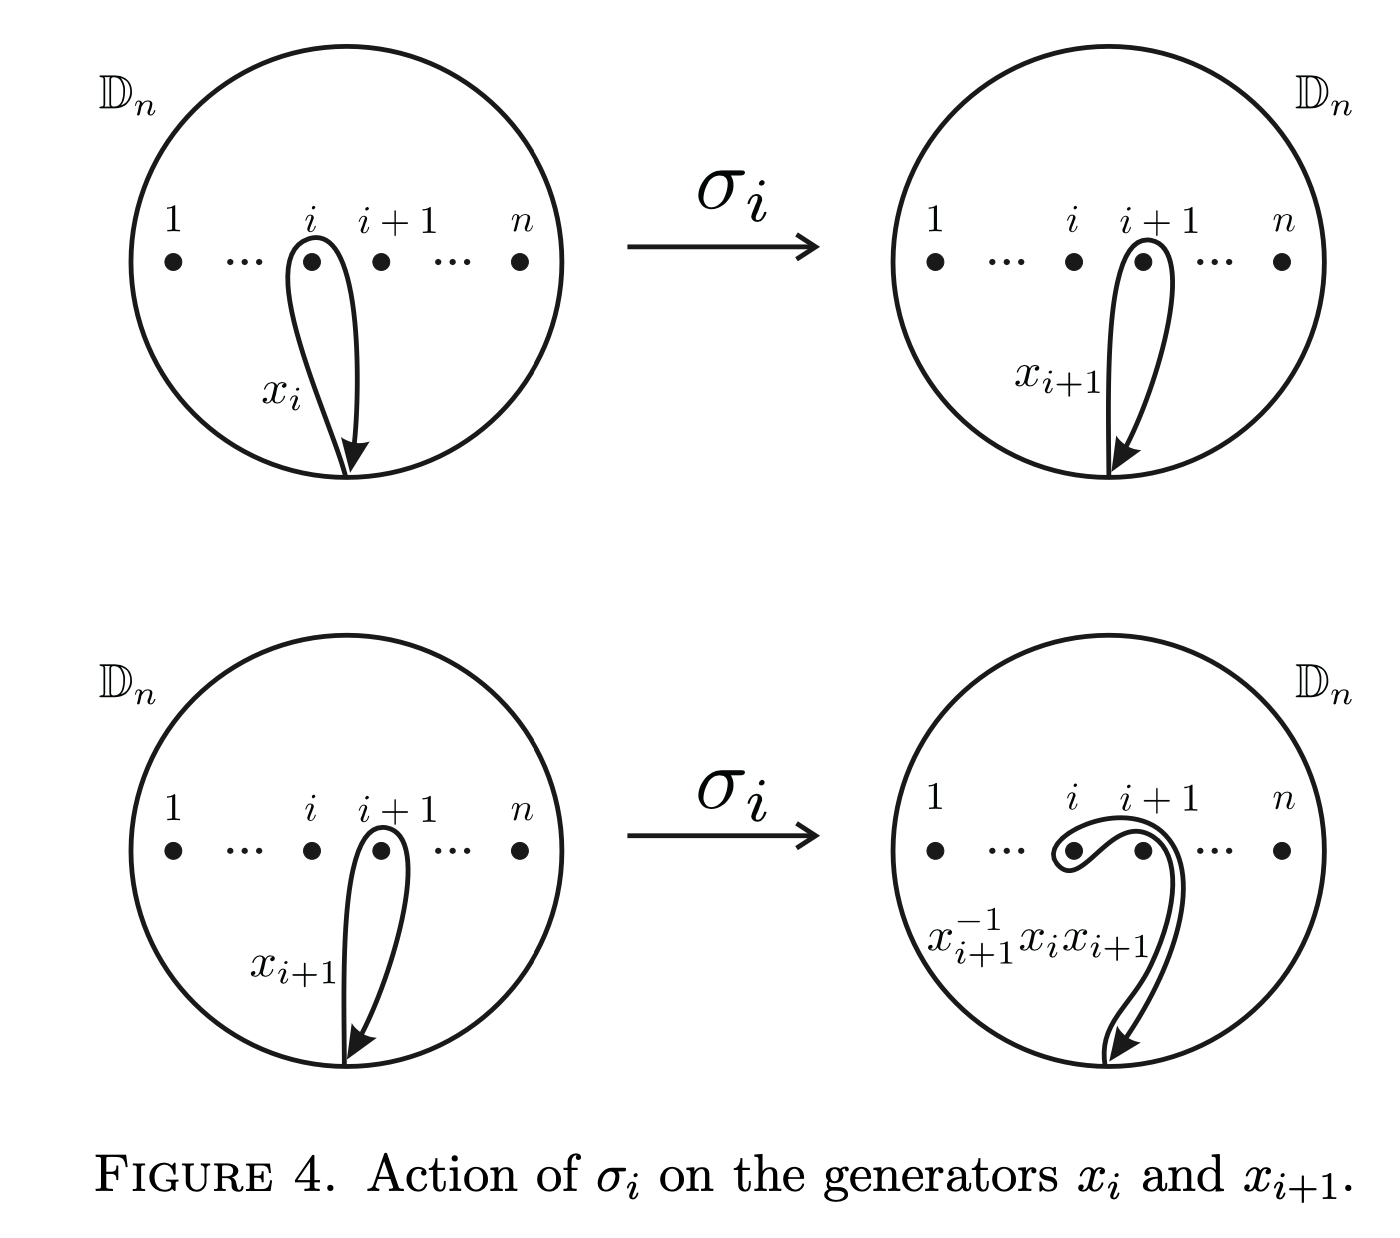
\includegraphics[width = .5\textwidth]{Gonzalez_Fig4_sigma_on_Dn.png}
%     \caption{\colorbox{red}{Gonzalez Figure 4}}\label{fig:sigma_on_Dn}
% \end{figure}

\begin{figure}[htbp]
    \centering
    \def\circleRadius{2.5cm}
\def\sep{\circleRadius*0.175}
\def\XOff{1.5*\circleRadius}
\def\YOff{-2.5*\circleRadius}

\pgfdeclarelayer{edgelayer}
\pgfdeclarelayer{nodelayer}
\pgfsetlayers{edgelayer,nodelayer,main}

\newcommand{\drawRegion}[3]{
        \begin{scope}[shift={#1}]
        \node[anchor=north west, font=\large] at (-\circleRadius, \circleRadius) {$\D_n$};

        \draw[ultra thick] (0,0) circle (\circleRadius);
        \filldraw [black] 
                (-\circleRadius + \sep,0) circle (2pt) node[above] {$1$}
                (\circleRadius - \sep,0) circle (2pt) node[above] {$n$}
                (-\sep,0) circle (2pt) node[above, yshift=.2*\sep] {$i$}
                (\sep,0) circle (2pt) node[above, yshift=.1*\sep] {$i+1$};
        \path (-\circleRadius/2,0) node {$\scalebox{1.5}{$\cdots$}$};
        \path (\circleRadius/2,0) node {$\scalebox{1.5}{$\cdots$}$};

        \ifx&#2&  % Check if #2 is empty
                % Do nothing if #2 is empty
        \else
                \draw[-latex, ultra thick] (0,-\circleRadius) .. controls #2 .. node[pos=0.1, left] {#3} (.05*\sep,-\circleRadius + 2.8452755906/2);
        \fi
        
        \filldraw [red] (0,-\circleRadius) circle (2pt);
        
        \end{scope}
}


\begin{tikzpicture}
        \drawRegion{(\XOff,0)}{(-1.425*\sep-.35*\circleRadius,0.39*\circleRadius) and  (-1.425*\sep+.35*\circleRadius,0.39*\circleRadius)}{$x_i$}
        
        \draw[-latex, ultra thick] (-\XOff + \circleRadius + 0.25cm, 0) -- node[above] {$\sigma_i$} (\XOff - \circleRadius - 0.25cm, 0);
        
        \drawRegion{(-\XOff,0)}{(1.3*\sep-.35*\circleRadius,0.39*\circleRadius) and  (1.3*\sep+.35*\circleRadius,0.39*\circleRadius)}{$x_{i+1}$}
        
        \drawRegion{(-\XOff,\YOff)}{(-1.425*\sep-.35*\circleRadius,0.39*\circleRadius) and  (-1.425*\sep+.35*\circleRadius,0.39*\circleRadius)}{$x_i$}

        \draw[-latex, ultra thick] (-\XOff + \circleRadius + 0.25cm, \YOff) -- node[above] {$\sigma_i$} (\XOff - \circleRadius - 0.25cm, \YOff);
        
        % \drawRegion{(\XOff,\YOff)}{}{}

        \begin{scope}[shift={(\XOff,\YOff)}]
                \node[anchor=north west, font=\large] at (-\circleRadius, \circleRadius) {$\D_n$};
        
                \draw[ultra thick] (0,0) circle (\circleRadius);
                \filldraw [black] 
                        (-\circleRadius + \sep,0) circle (2pt) node[above] {$1$}
                        (\circleRadius - \sep,0) circle (2pt) node[above] {$n$}
                        (-\sep,0) circle (2pt) node[above, yshift=.45*\sep] {$i$}
                        (\sep,0) circle (2pt) node[above, yshift=.3*\sep] {$i+1$};
                \path (-\circleRadius/2,0) node {$\scalebox{1.5}{$\cdots$}$};
                \path (\circleRadius/2,0) node {$\scalebox{1.5}{$\cdots$}$};
        
                \filldraw [red] (0,-\circleRadius) circle (2pt);

                \begin{pgfonlayer}{nodelayer}
                        \node (0) at (-1.5*\sep,.35*\sep ) {};
                        \node (1) at (0, -\circleRadius) {};
                        \node (2) at (1.5*\sep, -1.5*\sep) {$x_i x_{i+1}\iv{x_i}$};
                        \node (3) at (1.25*\sep, -.25*\sep) {};
                        \node (4) at (-.5*\sep, .35*\sep) {};
                        \node (5) at (.05*\sep, -\circleRadius + 2.8452755906/2) {};
                \end{pgfonlayer}
                \begin{pgfonlayer}{edgelayer}
                        \draw [in=105, out=-120, looseness=0.50, ultra thick] (0.center) to (1.center);
                        \draw [in=60, out=30, looseness=0.85, ultra thick] (3.center) to (0.center);
                        \draw [in=-150, out=-15, looseness=0.50, ultra thick] (4.center) to (3.center);
                        \draw [latex-, in=165, out=85, ultra thick] (5.center) to (4.center);
                \end{pgfonlayer}

                % \foreach \point in {0,1,3,4,5} {
                %         \fill[red] (\point) circle (2pt);
                %         \node[above right] at (\point) {\point};
                % }
        \end{scope}
        
        \draw[-latex, ultra thick] (-\XOff + \circleRadius + 0.25cm, 0) -- node[above] {$\sigma_i$} (\XOff - \circleRadius - 0.25cm, 0);
\end{tikzpicture}
    \caption{The action of $\sigma_i$ on the generators $x_i$ and $x_{i+1}$ as described by \cref{eq:rho_i,eq:rho_ip1,eq:rho_j}. The image of $x_i$ under $\sigma_i$ is verified visually in \cref{fig:sigma_on_x_i}}\label{fig:sigma_on_Dn}
\end{figure}

The automorphism $\rho_\beta$ is most simply defined in terms of the action of the standard generators of $B_n$ on the generators $x_1,\dots,x_n$ of $F_n$ (visualized as loops in $\D_n$). For each $i$, it follows that
\begin{align}
    &\rho_{\sigma_i}(x_{i}) = x_{i}x_{i+1} \iv{x_{i}}, \label{eq:rho_i}\\
    &\rho_{\sigma_i}(x_{i+1}) = x_{i}, \label{eq:rho_ip1}\\
    &\rho_{\sigma_i}(x_j) = x_j, \textrm{ for } j\neq i,i-1.\label{eq:rho_j}
\end{align}
Clearly, any two loops that are separated by at least one puncture will not interact while performing $\sigma_i$. The relations for adjacent loops can be verified graphically as illustrated in \cref{fig:sigma_on_Dn,fig:sigma_on_x_i}.
\begin{figure}[htbp]
    \centering
    \def\circleRadius{2.5cm}
\def\sep{\circleRadius*0.175}
\def\XOff{1.5*\circleRadius}
\def\YOff{-2.5*\circleRadius}

\usetikzlibrary{decorations.markings}

\pgfdeclarelayer{edgelayer}
\pgfdeclarelayer{nodelayer}
\pgfsetlayers{edgelayer,nodelayer,main}

\newcommand{\drawRegion}[3]{
        \begin{scope}[shift={#1}]
        \node[anchor=north west, font=\large] at (-\circleRadius, \circleRadius) {$\D_n$};

        \draw[ultra thick] (0,0) circle (\circleRadius);
        \filldraw [black] 
                (-\circleRadius + \sep,0) circle (2pt) node[above] {$0$}
                (\circleRadius - \sep,0) circle (2pt) node[above] {$n$}
                (-\sep,0) circle (2pt) node[above, yshift=.2*\sep] {$i$}
                (\sep,0) circle (2pt) node[above, yshift=.1*\sep] {$i+1$};
        \path (-\circleRadius/2,0) node {$\scalebox{1.5}{$\cdots$}$};
        \path (\circleRadius/2,0) node {$\scalebox{1.5}{$\cdots$}$};

        \filldraw [red] (0,-\circleRadius) circle (2pt);

        \ifx&#2&  % Check if #2 is empty
                % Do nothing if #2 is empty
        \else
                \draw[-latex, ultra thick] (0,-\circleRadius + 2.8452755906/2) .. controls #2 .. node[pos=0.1, left] {#3} (.05*\sep,-\circleRadius + 2.8452755906/2);
        \fi
        \end{scope}
}

\newcommand{\drawloop}[4]{\draw[ultra thick, postaction={decorate}, decoration={markings, mark= at position 0.75 with {\arrow{latex},sloped}}, #2] (0,-\circleRadius + 2.8452755906/2) .. controls #1 .. node[pos=#4, left] {#3} (.05*\sep,-\circleRadius + 2.8452755906/2);}

\newcommand{\rdrawloop}[4]{\draw[ultra thick, postaction={decorate}, decoration={markings, mark= at position 0.25 with {\arrowreversed{latex},sloped}}, #2] (0,-\circleRadius + 2.8452755906/2) .. controls #1 .. node[pos=#4, left] {#3} (.05*\sep,-\circleRadius + 2.8452755906/2);}


\begin{tikzpicture}
        \begin{scope}[shift={(-\XOff,0)}]
                \node[anchor=north west, font=\large] at (-\circleRadius, \circleRadius) {$\D_n$};
        
                \draw[ultra thick] (0,0) circle (\circleRadius);
                \filldraw [black] 
                        (-\circleRadius + \sep,0) circle (2pt) node[above] {$0$}
                        (\circleRadius - \sep,0) circle (2pt) node[above] {$n$}
                        (-\sep,0) circle (2pt) node[above, yshift=.2*\sep] {$i$}
                        (\sep,0) circle (2pt) node[above, yshift=.25*\sep] {$i+1$};
                \path (-\circleRadius/2,0) node {$\scalebox{1.5}{$\cdots$}$};
                \path (\circleRadius/2,0) node {$\scalebox{1.5}{$\cdots$}$};
        
                \filldraw [red] (0,-\circleRadius) circle (2pt);

                \begin{pgfonlayer}{nodelayer}
                        \node (0) at (.7*\sep,-.5*\circleRadius ) {};
                        \node (1) at (0, -\circleRadius + 2.8452755906/2) {};
                        \node (2) at (.5*\circleRadius, -2*\sep) {$\color{NavyBlue} x_{i+1}$};
                        \node (3) at (.9*\sep, .5*\sep) {};
                        \node (4) at (1.75*\sep, -.5*\circleRadius) {};
                        \node (5) at (.05*\sep, -\circleRadius + 2.8452755906/2) {};
                \end{pgfonlayer}
                \begin{pgfonlayer}{edgelayer}
                        \draw [in=30, out=-90, looseness=0.50, ultra thick, NavyBlue] (0.center) to (1.center);
                        \draw [in=90, out=-150, looseness=0.85, ultra thick, NavyBlue] (3.center) to (0.center);
                        \draw [in=20, out=80, looseness=0.50, ultra thick, NavyBlue, postaction={decorate}, decoration={markings, mark= at position .5 with {\arrowreversed{latex},sloped}}] (4.center) to (3.center);
                        \draw [in=-100, out=10, ultra thick, NavyBlue] (5.center) to (4.center);
                \end{pgfonlayer}
                
                % \foreach \point in {0,1,3,4,5} {
                %         \fill[red] (\point) circle (2pt);
                %         \node[above right] at (\point) {\point};
                % }

                \rdrawloop{(-1.4*\sep-.65*\circleRadius,0.7*\circleRadius) and  (-1.4*\sep+.55*\circleRadius,0.7*\circleRadius)}{purple}{$\iv{x_i}$}{.45}

                \drawloop{(-1.4*\sep-.35*\circleRadius,0.39*\circleRadius) and  (-1.4*\sep+.35*\circleRadius,0.39*\circleRadius)}{OliveGreen}{$x_i$}{.1}

        \end{scope}

        \begin{scope}[shift={(\XOff,0)}]
                \node[anchor=north west, font=\large] at (-\circleRadius, \circleRadius) {$\D_n$};
        
                \draw[ultra thick] (0,0) circle (\circleRadius);
                \filldraw [black] 
                        (-\circleRadius + \sep,0) circle (2pt) node[above] {$0$}
                        (\circleRadius - \sep,0) circle (2pt) node[above] {$n$}
                        (-\sep,0) circle (2pt) node[above, yshift=.3*\sep] {\small$i$}
                        (\sep,0) circle (2pt) node[above, xshift=0*\sep, yshift=.15*\sep] {\small$i+1$};
                \path (-\circleRadius/2,0) node {$\scalebox{1.5}{$\cdots$}$};
                \path (\circleRadius/2,0) node {$\scalebox{1.5}{$\cdots$}$};
        
                \filldraw [red] (0,-\circleRadius) circle (2pt);
                
                \begin{scope}[shift={(-.25*\sep,0)}]
                                \begin{pgfonlayer}{nodelayer}
                                \node (0) at (-1.75*\sep,-.15*\circleRadius ) {};
                                \node (1) at (.25*\sep, -\circleRadius + 2.8452755906/2) {};
                                % \node (2) at (.5*\circleRadius, -2*\sep) {$x_i x_{i+1}\iv{x_i}$};
                                \node (3) at (0*\sep, 1.5*\sep) {};
                                \node (4) at (2*\sep, -.05*\circleRadius) {};
                                \node (5) at (0*\sep, 0*\circleRadius) {};
                                \node (6) at (-1.2*\sep, .4*\sep) {};
                                \node (7) at (.3*\sep, -\circleRadius + 2.8452755906/2) {};

                                \node (ip1) at (2.5*\sep, -1.15*\sep) {$\color{NavyBlue} x_{i+1}$};
                                \node (i) at (-.4*\circleRadius, -2*\sep) {$\color{OliveGreen} x_{i}$};
                                \node (iiv) at (.1*\circleRadius, -3*\sep) {$\color{purple} \iv{x_{i}}$};
                        \end{pgfonlayer}
                        \begin{pgfonlayer}{edgelayer}
                                \draw [in=150, out=-90, looseness=0.50, ultra thick, OliveGreen] (0.center) to (1.center);
                                \draw [latex-, in=100, out=180, looseness=0.95, ultra thick, OliveGreen] (3.center) to (0.center);
                                \draw [in=0, out=90, looseness=0.9, ultra thick, NavyBlue] (4.center) to (3.center);
                                \draw [latex-, in=-100, out=-50, looseness=.9, ultra thick, NavyBlue] (5.center) to (4.center);
                                \draw [in=60, out=100, looseness=.9, ultra thick, purple] (5.center) to (6.center);
                                \draw [-latex, in=100, out=-110, looseness=.9, ultra thick, purple] (6.center) to (7.center);
                        \end{pgfonlayer}
                \end{scope}
                
                \foreach \point in {3,5} {
                                \fill[red] (\point) circle (1.5pt);
                                % \node[above right] at (\point) {\point};
                        }

                % \foreach \point in {0,1,3,4,5,6,7} {
                %         \fill[red] (\point) circle (1.5pt);
                %         \node[above right] at (\point) {\point};
                % }
        \end{scope}

        \begin{scope}[shift={(\XOff,\YOff)}]
                \node[anchor=north west, font=\large] at (-\circleRadius, \circleRadius) {$\D_n$};
        
                \draw[ultra thick] (0,0) circle (\circleRadius);
                \filldraw [black] 
                        (-\circleRadius + \sep,0) circle (2pt) node[above] {$0$}
                        (\circleRadius - \sep,0) circle (2pt) node[above] {$n$}
                        (-\sep,0) circle (2pt) node[above, yshift=.45*\sep] {$i$}
                        (\sep,0) circle (2pt) node[above, yshift=.3*\sep] {$i+1$};
                \path (-\circleRadius/2,0) node {$\scalebox{1.5}{$\cdots$}$};
                \path (\circleRadius/2,0) node {$\scalebox{1.5}{$\cdots$}$};
        
                \filldraw [red] (0,-\circleRadius) circle (2pt);

                \begin{pgfonlayer}{nodelayer}
                        \node (0) at (-1.5*\sep,.35*\sep ) {};
                        \node (1) at (0, -\circleRadius + 2.8452755906/2) {};
                        \node (2) at (1.5*\sep, -1.5*\sep) {$x_i x_{i+1}\iv{x_i}$};
                        \node (3) at (1.25*\sep, -.25*\sep) {};
                        \node (4) at (-.5*\sep, .35*\sep) {};
                        \node (5) at (.05*\sep, -\circleRadius + 2.8452755906/2) {};
                \end{pgfonlayer}
                \begin{pgfonlayer}{edgelayer}
                        \draw [in=105, out=-120, looseness=0.50, ultra thick] (0.center) to (1.center);
                        \draw [in=60, out=30, looseness=0.85, ultra thick] (3.center) to (0.center);
                        \draw [in=-150, out=-15, looseness=0.50, ultra thick] (4.center) to (3.center);
                        \draw [latex-, in=165, out=85, ultra thick] (5.center) to (4.center);
                \end{pgfonlayer}

        \end{scope}
        
        \draw[latex-latex, ultra thick] (-\XOff + \circleRadius + 0.25cm, 0) -- node[above] {\footnotesize Homotopic} node[below] {\tiny (Loop Concatenation)} (\XOff - \circleRadius - 0.25cm, 0);
        
        \draw[latex-latex, ultra thick] (\XOff, -\circleRadius - 0.1cm) -- (\XOff, \YOff+\circleRadius + 0.1cm);
\end{tikzpicture}
    \caption{Up to homotopy, the product $x_i x_{i+1} \iv{x_i}$ is visualized as the concatenation of the loops $x_i,x_{i+1},\iv{x_i}\in\pi_1(\D_n)$. In the top right diagram, small red dots are used indicate the (homotopically deformed) points of concatenation.}\label{fig:sigma_on_x_i}
\end{figure}

For any $\sigma_i$, $\rho_{\iv{\sigma_i}}$ is well-defined. It follows that for any braid $\beta\in B_n$, we can decompose $\rho_\beta$ the composition of the automorphisms of the standard generators $\sigma_1,\dots,\sigma_{n-1}$ and their inverses that make up $\beta$. 

Notice that for any $\sigma_i$, $\rho_{\sigma_i}(x_1\cdots x_n) = x_1\cdots x_n$. This is because the loop $x_1\cdots x_n$ in $\D_n$, encompassing all holes, is parallel to the boundary $\partial\D_n$. Thus, the action of $\sigma_i$ on $x_1\cdots x_n$ is trivial does not affect the structure of the loop up to isotopy. More generally, this implies that $\rho_\beta(x_1\cdots x_n) = x_1\cdots x_n$ for any $\beta\in B_n$. Paired with the observation that every generator is conjugate to another, Artin~\cite{Artin1947} showed that this is a necessary and sufficient condition for $\rho_\beta$ to be an automorphism of $F_n$.

\begin{theorem}
    An automorphism $f\in\aut{F_n}$ is equal to $\rho_\beta$ for some $\beta\in B_n$ if and only if
    \begin{enumerate}
        \item $f(x_i)$ is a conjugate of some $x_j$ for every $i\in\left\{ 1,\dots,n \right\}$, and
        \item $f(x_1\cdots x_n) = x_1\cdots x_n$.
    \end{enumerate}
\end{theorem}

In this interpretation of the braid group, we can express $B_n$ in terms of the standard generators:
\begin{equation}
    B_n = \left\langle \sigma_1,\dots,\sigma_{n-1} \;\middle|\;
    \begin{aligned}
        \sigma_i\sigma_j &= \sigma_j\sigma_i, & |i-j|&>1 \\
        \sigma_i\sigma_{i+1}\sigma_i &= \sigma_{i+1}\sigma_i\sigma_{i+1}, & |i-j|&=1
    \end{aligned}
    \right\rangle.
\end{equation}
The first condition that the standard generators commute if $|i-j|>1$ is easily verified by looking at the graphic of \cref{fig:sigma_on_x_i} in describing the property of the automorphism $\rho_{\sigma_i}(\sigma_j) = \sigma_j$. This follows by the fact that if two holes are non-adjacent, then the actions of $\sigma_i$ and $\sigma_j$ are mutually exclusive and thus commutative. The second condition on the standard generators is most easily verified in \cref{fig:YB_criterion_verification} by looking at the corresponding braids in $\R\times[0,1]$.
\begin{figure}[htbp]
    \centering
    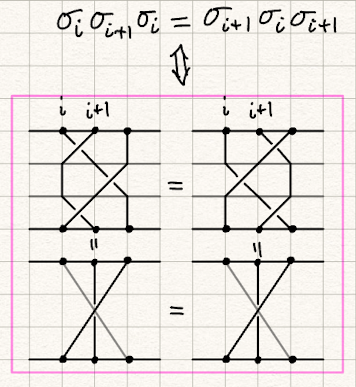
\includegraphics[width = .5\textwidth]{sketch_YB_citerion_verification.png}
    \caption{\colorbox{red}{Grayed-out strand indicates that it is behind all other strands.}}\label{fig:YB_criterion_verification}
\end{figure}

\section{The Burau Representation}
In the previous section, we defined a representation of the braid group $B_n$ as automorphisms of the free group $F_n$. This representation is clearly nonabelian. Likewise, the Artin generators of $B_n$ are nonabelian. Suppose we wish to abelianize the braid group. The details of the abelianization of $B_n$ would require a quotient by the commutator $\left[ a,b \right]=ab\iv{a}\iv{b}$.

Sparing the details, let $B_{n,ab} = B_n/\left[ B_n,B_n \right]$ be the abelianization of $B_n$, where $\left[ B_n,B_n \right]=\left\{ \left[ \beta_1,\beta_2 \right]\st\beta_1,\beta_2\in B_n \right\}$ is the commutator subgroup of $B_n$. Then, under the representation $\rho$ from \cref{sec:Aut_Fn}, the abelianization of \cref{eq:rho_i,eq:rho_ip1,eq:rho_j} become
\begin{align}
    x_i &\xmapsto{\sigma_i} \cancel{x_i} + x_{i+1} - \cancel{x_i} = x_{i+1} = \rho_{\iv{\sigma_i}}(x_i), \\
    x_{i+1} &\xmapsto{\sigma_i} x_i, \\
    x_j &\xmapsto{\sigma_i} x_j, \textrm{ for } j\neq i,i-1,
\end{align}
for each $i$. Thus, the generator $\sigma_i=\iv{\sigma_i}$, and corresponds to a transposition permutation in the symmetric group $S_n$. It follows that $B_{n,ab}\iso S_n$. In this current construction, the abelianization of the braid group results in a loss of complexity. This raises the question whether there exists such a reframing of the braid group that allows an abelian operation on the free generators while preserving the inequivalence of the Artin generators with their inverses.

First, we define a topological space that will aid in the desired construction.
\begin{definition}
    Let $X$ be a topological space. A \textit{covering} of $X$ is a space $\widetilde{X}$ together with a continuous map $p:\widetilde{X}\to X$ such that, for every $x\in X$, there exists a path-connected open neighborhood $U$ containing $x$ such that $\iv{p}(U)$ is a disjoint union of open sets in $\widetilde{X}$ where each component of $\iv{p}(U)$ is mapped homeomorphically onto $U$ by $p$. Each component of $\iv{p}(U)$ is called a \textit{sheet} of the covering, where the $i$-th sheet is denoted by $\sheet{X}{i}$, and total the number of sheets in $\iv{p}(U)$ is called the \textit{degree} of the covering.
\end{definition}

\begin{example}
    One of the simplest examples of a covering space is the covering of the circle $S^1$ by the real line by the parameterization map $p:\R\to S^1$ defined by $p(t)=\left( \cos t,\sin t \right)$. Clearly, there are infinitely many sheets in this covering.
\end{example}

\begin{example}
    A similar example is the covering of the circle $S^1$ through $p:\left[ 0,1 \right]\to S^1$ defined by $p(t) = e^{2\pi it}$. This defines a one-degree covering of $S^1$. If we instead let our domain be $\left[ 0,2 \right]$, then we have a two-degree covering of $S^1$.
\end{example}

With this topological tool, we construct a countably infinite-degree covering of the punctured disk $\D_n$, denoted $\widetilde{\D}_n$, which can be visualized as an infinite stack of copies of $\D_n$, with a slight modification to be explained shortly. Let $\sheet{\D}{n,i}$ denote the $i$-th sheet of $\widetilde{\D}_n$, and consider the base sheet our covering to be $\sheet{\D}{n,0}$.

We start this construction with a countably infinite stack of copies of $\D_n$. Then, for every $i\in\Z$, for each of the $n$ punctures on $\sheet{\D}{n,i}$, apply a cut from the hole to some point on the boundary of $\sheet{\D}{n,i}$, as illustrated in \cref{fig:D3_cuts} for the case when $n=3$. Each cut results in two edges, which will be referred to as the left edge and the right edge. Through a homeomorphic deformation, connect the left edge of $\sheet{\D}{n,i}$ to the corresponding right edge of $\sheet{\D}{n,i+1}$, and the right edge of $\sheet{\D}{n,i}$ to the left edge of $\sheet{\D}{n,i-1}$, for every cut on every sheet.

\begin{figure}[htbp]
    \centering
    % 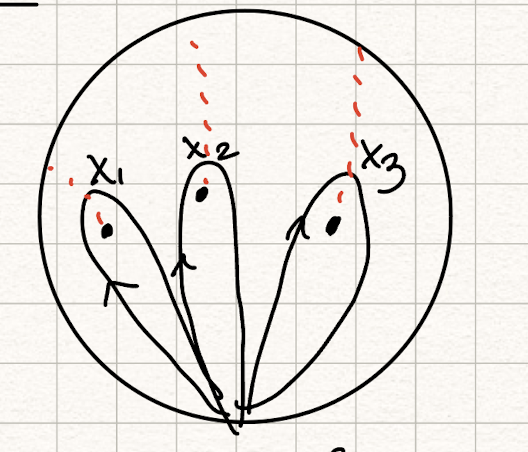
\includegraphics[width=.3\textwidth]{D3_cuts.png}
    % Suggested circle radius >= 3 cm
\usetikzlibrary{
        math,
        calc,
        % decorations.markings,
}

\def\circleRadius{3cm}
\def\sep{\circleRadius*0.175}
% \def\Off{.6}
% \def\eSep{.0005*\circleRadius}
% \def\cSep{1.2*\eSep}
\def\aSep{5} % degrees
\def\lA{130}
\def\cA{90}
\def\rA{50}

\begin{tikzpicture}[
] 
        \node[anchor=north west, font=\Large] at ({-1.15*\circleRadius}, {1.05*\circleRadius}) {$\sheet{\D}{n,i}$};

        \draw[ultra thick] (0,0) circle (\circleRadius);

        \tikzmath{
                coordinate \l, \r, \p, \b, \lI, \lO; real \aL, \aR;
                \aL1 = \lA+\aSep;
                \aR1 = \lA-\aSep;
                \aL2 = \cA+\aSep;
                \aR2 = \cA-\aSep;
                \aL3 = \rA+\aSep;
                \aR3 = \rA-\aSep;
                %
                \b = (0,-\circleRadius);
                \p1 = (-.5*\circleRadius,0);
                \p2 = (0,0);
                \p3 = (.5*\circleRadius,0);
                \l1 = (\aL1:\circleRadius);
                \r1 = (\aR1:\circleRadius);
                \l2 = (\aL2:\circleRadius);
                \r2 = (\aR2:\circleRadius);
                \l3 = (\aL3:\circleRadius);
                \r3 = (\aR3:\circleRadius);
                %
        %         Alternate method with cartesian coordinates
        %         \l1 = ({-(\Off + \eSep)*\circleRadius},{sqrt(1-(\Off + \eSep)^2) * \circleRadius});
        %         \l2 = (-\cSep*\circleRadius,{sqrt(1-(\cSep)^2) * \circleRadius});
        %         \l3 = ({(\Off - \eSep)*\circleRadius},{sqrt(1-(\Off - \eSep)^2) * \circleRadius});
        %         \r1 = ({-(\Off - \eSep)*\circleRadius},{sqrt(1-(\Off - \eSep)^2) * \circleRadius});
        %         \r2 = (\cSep*\circleRadius,{sqrt(1-(\cSep)^2) * \circleRadius});
        %         \r3 = ({(\Off + \eSep)*\circleRadius},{sqrt(1-(\Off + \eSep)^2) * \circleRadius});
        }
        
        % \foreach \i in {1,2,3} {
        %         \draw[white, line width=2pt] (\r\i) arc (atan2(\ry\i,\rx\i):atan2(\ly\i,\lx\i):\circleRadius);
        % }

        \foreach \i in {1,2,3} {
                \draw[white, line width=2pt] (\r\i) arc (\aR\i:\aL\i:\circleRadius);
        }

        % Alternate method with nodes
        % \node (l1) at ({\lA+\aSep}:\circleRadius) {};
        % \node (r1) at ({\lA-\aSep}:\circleRadius) {};
        % 
        % \node (l2) at ({\cA+\aSep}:\circleRadius) {};
        % \node (r2) at ({\cA-\aSep}:\circleRadius) {};
        % 
        % \node (l3) at ({\rA+\aSep}:\circleRadius) {};
        % \node (r3) at ({\rA-\aSep}:\circleRadius) {};

        \foreach \i in {1,2,3} {
                \coordinate (lI\i) at ($(\p\i)!0.5!(\l\i)$);
                \coordinate (lO\i) at ($(\p\i)!0.5!(\r\i)$);

                \fill[cyan] (\l\i) circle (.75pt);
                \fill[purple] (\r\i) circle (.75pt);
        }

        \node at (\l2) [left, yshift=-.3*\circleRadius, xshift=.04*\circleRadius, cyan] {$\substack{\textrm{Left} \\ \textrm{Edge}}$};
        \node at (\r2) [right, yshift=-.3*\circleRadius, xshift=-.04*\circleRadius, purple] {$\substack{\textrm{Right} \\ \textrm{Edge}}$};

        \draw [out=135, in=-140, looseness=.65, line width= 1.4, decoration={markings, mark= at position 0.6 with {\arrow{latex},sloped}}, postaction={decorate}] (\b) to (lI1);
        

        \draw [out=80, in=-170, looseness=.65, line width= 1.4, decoration={markings, mark= at position 0.6 with {\arrowreversed{latex},sloped}}, postaction={decorate}] (\b) to (lI3);

        \draw [out=110, in=-110, looseness=0, ultra thick, cyan] (\p1) to (\l1);
        \draw [out=110, in=-110, looseness=0, ultra thick, cyan] (\p2) to (\l2);
        \draw [out=110, in=-110, looseness=0, ultra thick, cyan] (\p3) to (\l3);
        
        \draw [out=80, in=-80, looseness=0, ultra thick, purple] (\p1) to (\r1);
        \draw [out=80, in=-80, looseness=0, ultra thick, purple] (\p2) to (\r2);
        \draw [out=80, in=-80, looseness=0, ultra thick, purple] (\p3) to (\r3);

        \foreach \i in {1,2,3} {
                \fill[black] (\p\i) circle (2pt);
                \node[above, yshift=-.15*\sep, xshift=.45*\sep] at (\p\i) {$\i$};
        }

        % base point for loop/arrow
        \filldraw [red] (\b) circle (2pt) node[below] {$t^i\zeta$};
\end{tikzpicture}

    \caption{
        % In the case of $\D_3$, this figure demonstrates how the cuts are applied across each of the three punctures for each sheet in the covering $\widetilde{\D}_3$. The power of $t$ in the base point label $t^j\zeta$ indicates that we are on the $j$-th sheet of the covering.
        For the covering of $\D_3$, we observe the $i$-th sheet of $\widetilde{\D}_3$ with the cuts applied across each of the three punctures. The base point of the loop is indicated by the red dot, and labelled as $t^i\zeta$. The power of $t$ indicates that we are on the $i$-th sheet of the covering. The portions of three different loops are drawn to illustrate the behavior of loops as they pass through various edges on $\sheet{\D}{3,i}$. The loop that would traditionally be $x_1$ is labeled by $t^i x_1$ to indicate that it's starting on the $i$-th sheet. When it passes through the left edge corresponding to this puncture labeled with a 1, it traverses up to the sheet $\sheet{\D}{3,i+1}$ and ends at base point $t^{i+1}\zeta$. Similarly, the loop that started on $\sheet{\D}{3,i-1}$ and passed through the left edge of puncture 2 ends up coming out of the right edge of puncture 2 on $\sheet{\D}{3,i}$ and ends at the base point $t^i\zeta$. This loop is labeled by the starting sheet, so it is $t^{i-1}x_2$. Finally, the loop that started on $\sheet{\D}{3,i+1}$ and passed through the right edge of puncture 3 ends up coming out of the left edge of puncture 3 on $\sheet{\D}{3,i}$ and is therefore labeled by $-t^{i+1}x_3$, with the negative sign indicating that the loop direction is reversed.
    }\label{fig:D3_cuts}
\end{figure}

Now, viewing a single sheet, say $\sheet{\D}{n,0}$, from above, when a loop with base point $\tilde{\zeta}_0$ passes through a cut from the left, it traverses up to the next sheet, and ends at the base point $\tilde{\zeta}_1$. Similarly, a loop passing through a cut from the right ends at the base point $\tilde{\zeta}_{-1}$, on the sheet $\sheet{\D}{n,-1}$ below $\sheet{\D}{n,0}$. To keep track of the starting sheet of a loop, we use a free parameter $t$. For example, a loop $\gamma$ that starts on $\sheet{\D}{n,j}$ would be written $t^j \gamma$, for $j\in\Z$. Notice that the substitution of a complex number for the free parameter $t$ results in a possibly finite degree covering. As an example, if we set $t$ to an $n$-th root of unity, then we obtain an $n$-th degree covering of $\D_n$. For the purposes of this construction, we will keep $t$ as a free parameter for now.{ }\cref{fig:D3_cuts} demonstrates how loops interact with the cuts on different sheets. The following example describes the action of the standard generators of $B_3$ on the covering space $\widetilde{\D}_3$.

\begin{example}\label{ex:Burau_D3}
    Consider the case when $n=3$. Then we have the corresponding covering space $\widetilde{\D}_3$ of $\D_3$. See \cref{fig:D3_cuts} for the view of a single sheet with various loops interacting with the cuts on the sheet. The actions of the standard generators of $B_3$ in $\pi_1(\D_3)$ are known, and can be visually understood in \cref{fig:sigma_on_Dn}. In the context of the covering space $\widetilde{\D}_3$, the action of the generators $\sigma_1$ and $\sigma_2$ is observed by reducing the visualization to only the base points on each sheet and the loops themselves. This can be seen in \cref{fig:Burau_D3} for the case of $\sigma_1$.
    
    \begin{figure}[htbp]
        \centering
        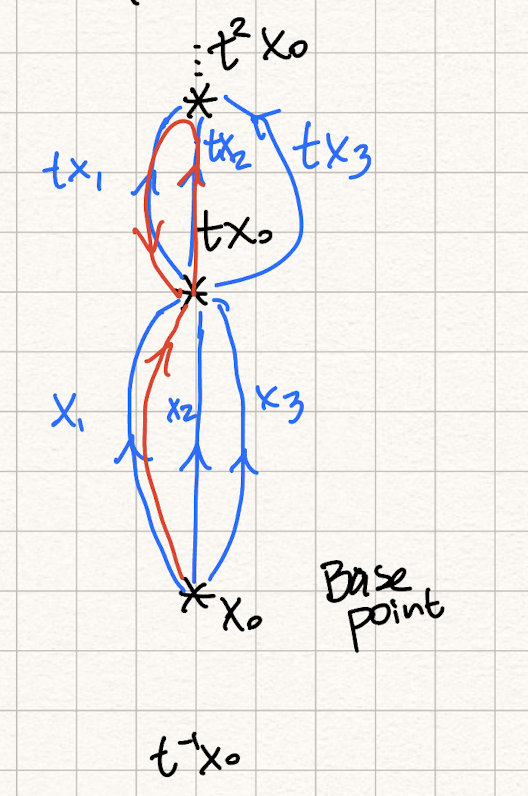
\includegraphics[width = .3\textwidth]{Burau_D3.png}
    %     % \input{TikZ/D3_covering.tikz}
        \caption{\colorbox{red}{CAPTION}}\label{fig:Burau_D3}
    \end{figure}

    Now, we can express loop concatenation as an abelian operation, where \cref{eq:rho_i,eq:rho_ip1,eq:rho_j} become
    \begin{align}
        x_1 \xmapsto{\sigma_1} x_1 + tx_2 - tx_1 &= (1-t)x_1 + tx_2, \\
        x_{2} &\xmapsto{\sigma_1} x_1, \\
        x_3 &\xmapsto{\sigma_1} x_3.
    \end{align}
    Consider the vector $\begin{bmatrix}
        x_1 \\ x_2 \\ x_3
    \end{bmatrix}$. Then the action of $\sigma_1$ on the loops $x_1,x_2,x_3$ is realized by the matrix $\begin{bmatrix}
        1-t & t & 0 \\ 1 & 0 & 0 \\ 0 & 0 & 1
    \end{bmatrix}$ since
    \begin{equation}
        \begin{bmatrix}
            1-t & t & 0 \\ 1 & 0 & 0 \\ 0 & 0 & 1
        \end{bmatrix}\begin{bmatrix}
            x_1 \\ x_2 \\ x_3
        \end{bmatrix} = \begin{bmatrix}
            (1-t)x_1 + tx_2 \\ x_1 \\ x_3
        \end{bmatrix}.
    \end{equation}
    The action of $\sigma_2$ is obtained similarly, where
    \begin{equation}
        \sigma_2 \mapsto \begin{bmatrix}
            1 & 0 & 0 \\ 0 & 1-t & t \\ 0 & 1 & 0
        \end{bmatrix}.
    \end{equation}
    Notice that these matrices have entries in the ring of Laurent polynomials, $\Lambda=\Z[t,\iv{t}]$.
\end{example}

Clearly, the result from \cref{ex:Burau_D3} generalizes to the case of braids on $n$ strands. Fix $n>1$. Let $I_k$ denote the $k\times k$ dimensional identity matrix, and let
\begin{equation}
    U=\begin{bmatrix}
        1-t & t \\ 1 & 0
    \end{bmatrix}.
\end{equation} 
For $i\in\left\{ 1,\dots,n-1 \right\}$, the action of $\sigma_i$ on $\pi_1\left( \widetilde{\D}_n \right)$ is realized as an $n\times n$ matrix with entries in $\Lambda = \Z[t,\iv{t}]$. 

The Burau representation of $B_n$ is then defined by:
\begin{align}
    \psi_n:B_n&\to\textrm{GL}_n(\Lambda) \\
    \sigma_i &\mapsto \begin{bmatrix}
        I_{i-1} & 0 & 0 \\
        0 & U & 0 \\
        0 & 0 & I_{n-i-1}
    \end{bmatrix}.
\end{align}
\colorbox{red}{Show invertible/inverse?}

The Burau representation need only be defined on the standard generators, since any braid $\beta\in B_n$ decomposes into a product of $\sigma_1,\dots,\sigma_{n-1}$ and their inverses. Notice that if we set $t\to 1$, we recover the defining representation of $S_n$, as expected when we use a degree 1 covering space of $\D_n$ and force the action of the generators to be abelian. Furthermore, by direct computation, it follows that
\begin{align}
    \psi_n(\sigma_i)\psi_n(\sigma_j) &= \psi_n(\sigma_j)\psi_n(\sigma_i) \textrm{ for } |i-j|>1, \\
    \psi_n(\sigma_i)\psi_n(\sigma_{i+1})\psi_n(\sigma_i) &= \psi_n(\sigma_{i+1})\psi_n(\sigma_i)\psi_n(\sigma_{i+1}) \textrm{ for } |i-j|=1.
\end{align}

\chapter{Anyons}\label{ch:anyons}

The first few sections come from \cite{Khare2005}.

\section{Two Non-Interacting Anyons}\label{sec:non_int}

The interaction term in the Lagrangian for two anyons due to the braiding of the anyons is given by
\begin{equation}
    \mathcal{L}_{\text{int}} = \hbar\alpha\dot{\phi},
\end{equation}
where a dot indicates a total time derivative $\frac{d}{dt}$ and $\phi = \arctan\left( \frac{y_2-y_1}{x_2-x_1} \right)$ is the relative angle between the two anyons with positions $\vec{r}_1=(x_1,y_1)$ and $\vec{r}_2=(x_2,y_2)$. As in the previous section, $\alpha\in\left[ 0,1 \right]$ is the \textit{winding angle} or braiding statistic of the anyons. The parameter $\alpha$ can also be thought of as an angle modulo $\pi$. Though the relative angle $\phi$ is ambiguous for identical particles, the derivative $\frac{d\phi}{dt}=\dot{\phi}$ is well-defined.

Notice that if we take $\alpha\to 0$, the interaction term vanishes as expected for bosons. Similarly, for $\alpha>0$, $\phi$ becomes singular if $\vec{r}_1 = \vec{r_2}$, which motivates the Pauli exclusion principle for fermions. In fact, this means that for any $\alpha>0$, the corresponding anyons exhibit some form of the Pauli exclusion principle.

The classical kinetic energy of this system is
\begin{equation}
    T = \frac{1}{2}m\left( {\vd{r}_1}^2 + {\vd{r}_2}^2 \right),
\end{equation}
as expected. Then the Lagrangian for this system is
\begin{align}
    \mathcal{L}\left( \vd{r}_1,\vd{r}_2, \dot{\phi} \right) &= T + \mathcal{L}_{\text{int}} = \frac{1}{2}m\left( {\vd{r}_1}^2 + {\vd{r}_2}^2 \right) + \hbar\alpha\dot{\phi},
\end{align}
which can also be viewed as the Lagrangian for 2 interacting bosons/fermions.

We can redefine the Lagrangian in terms of the relative and center-of-mass coordinates
\begin{align}
    \vec{R} &= \frac{\vec{r}_1+\vec{r}_2}{2}, \\
    \vec{r} &= \vec{r}_1-\vec{r}_2,
\end{align}
where $\vec{r}$ is the relative position vector and $\vec{R}$ is the center-of-mass position vector of the two anyons. Note that we are assuming that the mass of the two particles are equal ($m_1=m_2$). Classically, the momentum of a particle is given by the product of its mass and velocity. Then the corresponding center-of-mass and relative momenta:
\begin{align}
    \vec{P} &= 2m\vd{R} = 2m \frac{\vec{r}_1+\vec{r}_2}{2} = m\vd{r}_1 + m\vd{r}_2 = \vec{p}_1 + \vec{p}_2, \\
    \vec{p} &= \mu\vd{r} = \frac{m}{2}\left( \vd{r}_1-\vd{r}_2 \right) = \frac{\vec{p}_1 - \vec{p}_2}{2},
\end{align}
where $m$ is the mass of each anyon and $\mu$ is the reduced mass of the system.

With this in mind, we derive the following identity:
\begin{align}
    \vd{R} + \frac{1}{4}\vd{r} &= \frac{{\left( \vd{r}_1 + \vd{r}_2 \right)}^2}{4} + \frac{{\left( \vd{r}_1 - \vd{r}_2 \right)}^2}{4} = \frac{{\vd{r}_1}^2 + {\vd{r}_2}^2}{2}.
\end{align}
Thus, the Lagrangian decomposes into relative and center-of-mass components upon making the substitution from the above identity:
\begin{align}
    \mathcal{L} = \underbrace{m\vd{R}^2}_{\mathcal{L}_R} + \underbrace{\frac{m{\vd{r}}^{\;2}}{4} + \hbar\alpha\dot{\phi}}_{\mathcal{L}_r},
\end{align}
where the squared velocities indicate magnitude squared. Observe that the center-of-mass component of the Lagrangian, $\mathcal{L}_R$, is independent of the braiding parameter $\alpha$. We can further simplify the relative component of the Lagrangian, $\mathcal{L}_r$, by noting that we can briefly write the coordinate $\vec{r}$ in polar form by representing it as a complex number $\vec{r} =r e^{i\phi}$. It follows that
\begin{align}
    \size{\vd{r}(r,\phi)}^2 = \size{\frac{d}{dt}\vec{r}(r,\phi)}^2 = \size{\left( \dot{r} + ir\dot{\phi} \right)e^{i\phi}}^2 = \dot{r}^2 + r^2\dot{\phi}^2.
\end{align}
Hence, we rewrite the relative component of the Lagrangian as
\begin{align}
    \mathcal{L}_r = \frac{m\left( \dot{r}^2 + r^2\dot{\phi}^2 \right)}{4} + \hbar\alpha\dot{\phi}.\label{eq:basic_Lr}
\end{align}

Recall that the classical relative angular momentum can be described by:
\begin{equation}
    p_\phi = \frac{d\mathcal{L}}{d\dot{\phi}} = \frac{mr^2}{2}\dot{\phi} + \hbar\alpha.
\end{equation}

Now, the Hamiltonian for this system can be constructed:
\begin{align}
    \mathcal{H} 
    &= P\dot{R} + p_r\dot{r} + p_\phi\dot{\phi} - \mathcal{L} \nonumber \\
    &= \frac{P^2}{4m} + \frac{p_r^{2}}{m} + \frac{mr^2}{4} {p_\phi}^2 \nonumber \\
    &= \frac{P^2}{4m} + \frac{p_r^{2}}{m} + \frac{{\left( p_\phi - \hbar\alpha \right)}^2}{mr^2}.
\end{align}
Once again, the center-of-mass component of the Hamiltonian is independent of $\alpha$, and so we can focus on the relative component of the Hamiltonian, which is
\begin{equation}
    \mathcal{H}_r = \frac{p_r^{2}}{m} + \frac{{\left( p_\phi - \hbar\alpha \right)}^2}{mr^2}.\label{eq:basic_Hr}
\end{equation}
For the purposes of this work, we need not carry out to find the energy eigenstates corresponding to the quantum operator of this relative Hamiltonian. More about this is found in~\cite{Khare2005}.


\section{Anyons in Harmonic Potential}\label{sec:mult_harmonic}

The Hamiltonian for this system requires modification from previous sections when the anyons are placed in a harmonic potential. The potential energy of a 2-anyon system is given by
\begin{equation}
    V(\vec{r}_1,\vec{r}_2) = \frac{1}{2}m\omega^2\left( {\vec{r}_1}^{\;2} + {\vec{r}_2}^{\;2} \right) = m\omega^2\left( {\vec{R}}^2 + \frac{1}{4}{\vec{r}}^{\;2} \right),
\end{equation}
where $\omega$ is the angular frequency of the harmonic potential. We can make the same substitution as in the previous section to write the potential in terms of the relative and center-of-mass coordinates. As is the recurring theme, the center-of-mass component of the potential has no dependence on the braiding parameter $\alpha$, and corresponds to a 2-dimensional quantum harmonic oscillator problem for a particle of mass $2m$.

Note that we can generalize \cref{eq:basic_Lr} (now omitting the subscript $r$) to an $N$-anyon system in a harmonic potential by writing
\begin{equation}
    \mathcal{L} = \sum_{i=1}^{N}\frac{m}{2}\vd{r}_i^{\;2} + \hbar\alpha\sum_{i\neq j}\dot{\phi}_{ij} - \frac{m\omega^2}{2}\sum_{i=1}^{N}{\vec{r}_i}^{\;2},
\end{equation}
where $\phi_{ij} = \arctan\left( \frac{y_i-y_j}{x_i-x_j} \right)$ is the relative angle between anyons $i$ and $j$. For brevity, we write $x_{ij} = x_i-x_j$ and $y_{ij} = y_i-y_j$ to denote the relative coordinates between the anyons.

More generally, let $\vec{r}_{ij} = \vec{r}_i - \vec{r}_j$ be the relative coordinate between anyons $i$ and $j$, and define $r_{ij}^2 = \size{{\vec{r}_{ij}}}^2$. Then we can solve directly for $\dot{\phi}_{ij}$ as follows:
\begin{align*}
    \dot{\phi}_{ij} = \frac{d\phi_{ij}}{dt} = \frac{d}{dt}\arctan\left( \frac{y_{ij}}{x_{ij}} \right)
        &= \frac{\frac{d}{dt}\left( \frac{y_{ij}}{x_{ij}} \right)}{1+{\left( \frac{y_{ij}}{x_{ij}} \right)}^2} \\
        &= \frac{x_{ij}\dot{y}_{ij} - \dot{x}_{ij}y_{ij}}{x_{ij}^2\left[ 1+{\left( \frac{y_{ij}}{x_{ij}} \right)}^2 \right]} \\
        &= \frac{x_{ij}\dot{y}_{ij} - \dot{x}_{ij}y_{ij}}{x_{ij}^2 + y_{ij}^2} \\
        &= \frac{\vec{r}_{ij}\times\vd{r}_{ij}}{r_{ij}^2}.
\end{align*}

Setting $\hbar=1$, we can rewrite the Lagrangian as~\cite{Date2003}
\begin{equation}
    \mathcal{L} = \frac{m}{2}\sum_{i=1}^{N}\left[ \vd{r}^{\;2} - \omega^2\vec{r}_i^{\;2} \right] + \alpha\sum_{i<j}^{N}\frac{\vec{r}_{ij}\times\vd{r}_{ij}}{{r}_{ij}^{\;2}}.\label{eq:compact_L}
\end{equation}

% To obtain the general Hamiltonian for $N$ anyons in a harmonic well, we need to better characterize the anyons~\cite{Date2003,Khare2005}. First, suppose that each (identical) anyon has 

% Now the Hamiltonian includes the potential energy:
% \begin{align}
%     % \mathcal{H} = \frac{p_r^{2}}{m} + \frac{{\left( p_\phi - \hbar\alpha \right)}^2}{mr^2} + V(\vec{r}) = \frac{p_r^{2}}{m} + \frac{{\left( p_\phi - \hbar\alpha \right)}^2}{mr^2} + \frac{m\omega^2}{4}\vec{r}^{\;2}.\label{eq:HO_Hr}
% \end{align}

The vector (gauge) potential associated with the $i$-th anyon is given by~\cite{Khare2005,Date2003,Moriyasu1983}
\begin{align}
    \vec{A}_i(\vec{r}_i) &= \alpha\sum_{j\neq i}\frac{\hat{z}\times \vec{r}_{ij}}{r_{ij}^2} = \alpha\sum_{j\neq i}\frac{-y_{ij}\hat{x} + x_{ij}\hat{y}}{r_{ij}^2}, \label{eq:gauge}
\end{align}
where $\hat{z}$ is the unit vector perpendicular to the $r_{ij}$-plane. Here, $\alpha$ serves as the coupling constant, which dictates the strength of the interaction between anyons in our system. This will allow us to consolidate the interactions between the anyons into the Hamiltonian.

As an aside, for fermions, such as electrons, $\alpha=1$ corresponds to the strongest form of coupling in the way described above. On the other hand, for bosons ($\alpha=0$), we have no coupling between particles, which is reflected in \cref{eq:gauge}.

For the $i$-th anyon, the contribution to the Hamiltonian can be written as
\begin{align}
    \mathcal{H}_i = \frac{1}{2m}{(\vec{p}_i - \vec{A}_i(\vec{r}_i))}^2 + \frac{m\omega^2}{2}{r}_i^{2},
\end{align}
where the $p_i - A_i(\vec{r}_i)$ term represents the canonical momentum of the system. This is a required modification since we must account for the motion of the anyons in the presence of the gauge potential in addition to their mechanical momentum.

Then, with only essential coupling  (minimal prescription) between the anyons by means of the gauge potential, the Hamiltonian for the $N$-anyon system in a harmonic potential is given by
\begin{align}
    \mathcal{H} = \frac{1}{2m} \sum_{i=1}^{N}{(\vec{p}_i - \vec{A}_i(\vec{r}_i))}^2 + \frac{m\omega^2}{2}\sum_{i=1}^{N}{r}_i^{2}. \label{eq:min_prescription_H}
\end{align}

Substituting \cref{eq:gauge} into \cref{eq:min_prescription_H}, this gives rise to
\begin{equation}
    \mathcal{H} = \frac{1}{2m}\sum_{i=1}^{N}\vec{p}_i^{\;2} + \frac{m\omega^2}{2}\sum_{i=1}^{N}\vec{r}_i^{\;2} - \frac{\alpha}{2m}\sum_{j\neq i}^{N}\frac{\vec{\ell}_{ij}}{r_{ij}^2} + \frac{\alpha^2}{2m}\sum_{j,k\neq i}^{N}\frac{\vec{r}_{ij}\cdot\vec{r}_{ik}}{r_{ij}^2r_{ik}^2},\label{eq:full_H}
\end{equation}
where $\vec{\ell}_{ij} = (\vec{r}_i-\vec{r}_j)\times(\vec{p}_i-\vec{p}_j)$ is the relative angular momentum of anyon $i$ and $j$.

\subsection{Notes}
\subsubsection{Hamiltonian Terms}
The last term in \cref{eq:full_H} is the result of squaring the canonical momentum in \cref{eq:min_prescription_H}. For example, let's isolate one set of the terms. Fix $i$. Then,
\begin{align*}
    {(\vec{p}_i - \vec{A}_i(\vec{r}_i))}^2 = {p}_i^{2} - 2\vec{p}_i\cdot\vec{A}_i(\vec{r}_i) + \vec{A}_i^{\;2}(\vec{r}_i).
\end{align*}

By \cref{eq:gauge}, we have
\begin{align*}
    \vec{A}_i^{\;2}(\vec{r}_i) = {\left( \alpha\sum_{j\neq i}\frac{-y_{ij}\hat{x} + x_{ij}\hat{y}}{r_{ij}^2} \right)}^2 = \alpha^2\sum_{j,k\neq i}\frac{y_{ij}y_{ik} + x_{ij}x_{ik}}{r_{ij}^2r_{ik}^2} = \alpha^2\sum_{j,k\neq i}\frac{\vec{r}_{ij}\cdot\vec{r}_{ik}}{r_{ij}^2r_{ik}^2}.
\end{align*}

\subsubsection{Connecting Lagrangian to Hamiltonian}
The connection between \cref{eq:compact_L} and \cref{eq:gauge} is the multiplication of $\vec{A}_i(\vec{r}_i)$ by $\vd{r}_{ij}$, as is done when constructing the Hamiltonian.

\chapter{tikz test}\label{ch:tikz_test}

\begin{figure}[htbp]
    \centering
    \def\circleRadius{2.5cm}
\def\sep{\circleRadius*0.175}
\def\XOff{1.5*\circleRadius}
\def\YOff{-2.5*\circleRadius}

\pgfdeclarelayer{edgelayer}
\pgfdeclarelayer{nodelayer}
\pgfsetlayers{edgelayer,nodelayer,main}

\newcommand{\drawRegion}[3]{
        \begin{scope}[shift={#1}]
        \node[anchor=north west, font=\large] at (-\circleRadius, \circleRadius) {$\D_n$};

        \draw[ultra thick] (0,0) circle (\circleRadius);
        \filldraw [black] 
                (-\circleRadius + \sep,0) circle (2pt) node[above] {$1$}
                (\circleRadius - \sep,0) circle (2pt) node[above] {$n$}
                (-\sep,0) circle (2pt) node[above, yshift=.2*\sep] {$i$}
                (\sep,0) circle (2pt) node[above, yshift=.1*\sep] {$i+1$};
        \path (-\circleRadius/2,0) node {$\scalebox{1.5}{$\cdots$}$};
        \path (\circleRadius/2,0) node {$\scalebox{1.5}{$\cdots$}$};

        \ifx&#2&  % Check if #2 is empty
                % Do nothing if #2 is empty
        \else
                \draw[-latex, ultra thick] (0,-\circleRadius) .. controls #2 .. node[pos=0.1, left] {#3} (.05*\sep,-\circleRadius + 2.8452755906/2);
        \fi
        
        \filldraw [red] (0,-\circleRadius) circle (2pt);
        
        \end{scope}
}


\begin{tikzpicture}
        \drawRegion{(\XOff,0)}{(-1.425*\sep-.35*\circleRadius,0.39*\circleRadius) and  (-1.425*\sep+.35*\circleRadius,0.39*\circleRadius)}{$x_i$}
        
        \draw[-latex, ultra thick] (-\XOff + \circleRadius + 0.25cm, 0) -- node[above] {$\sigma_i$} (\XOff - \circleRadius - 0.25cm, 0);
        
        \drawRegion{(-\XOff,0)}{(1.3*\sep-.35*\circleRadius,0.39*\circleRadius) and  (1.3*\sep+.35*\circleRadius,0.39*\circleRadius)}{$x_{i+1}$}
        
        \drawRegion{(-\XOff,\YOff)}{(-1.425*\sep-.35*\circleRadius,0.39*\circleRadius) and  (-1.425*\sep+.35*\circleRadius,0.39*\circleRadius)}{$x_i$}

        \draw[-latex, ultra thick] (-\XOff + \circleRadius + 0.25cm, \YOff) -- node[above] {$\sigma_i$} (\XOff - \circleRadius - 0.25cm, \YOff);
        
        % \drawRegion{(\XOff,\YOff)}{}{}

        \begin{scope}[shift={(\XOff,\YOff)}]
                \node[anchor=north west, font=\large] at (-\circleRadius, \circleRadius) {$\D_n$};
        
                \draw[ultra thick] (0,0) circle (\circleRadius);
                \filldraw [black] 
                        (-\circleRadius + \sep,0) circle (2pt) node[above] {$1$}
                        (\circleRadius - \sep,0) circle (2pt) node[above] {$n$}
                        (-\sep,0) circle (2pt) node[above, yshift=.45*\sep] {$i$}
                        (\sep,0) circle (2pt) node[above, yshift=.3*\sep] {$i+1$};
                \path (-\circleRadius/2,0) node {$\scalebox{1.5}{$\cdots$}$};
                \path (\circleRadius/2,0) node {$\scalebox{1.5}{$\cdots$}$};
        
                \filldraw [red] (0,-\circleRadius) circle (2pt);

                \begin{pgfonlayer}{nodelayer}
                        \node (0) at (-1.5*\sep,.35*\sep ) {};
                        \node (1) at (0, -\circleRadius) {};
                        \node (2) at (1.5*\sep, -1.5*\sep) {$x_i x_{i+1}\iv{x_i}$};
                        \node (3) at (1.25*\sep, -.25*\sep) {};
                        \node (4) at (-.5*\sep, .35*\sep) {};
                        \node (5) at (.05*\sep, -\circleRadius + 2.8452755906/2) {};
                \end{pgfonlayer}
                \begin{pgfonlayer}{edgelayer}
                        \draw [in=105, out=-120, looseness=0.50, ultra thick] (0.center) to (1.center);
                        \draw [in=60, out=30, looseness=0.85, ultra thick] (3.center) to (0.center);
                        \draw [in=-150, out=-15, looseness=0.50, ultra thick] (4.center) to (3.center);
                        \draw [latex-, in=165, out=85, ultra thick] (5.center) to (4.center);
                \end{pgfonlayer}

                % \foreach \point in {0,1,3,4,5} {
                %         \fill[red] (\point) circle (2pt);
                %         \node[above right] at (\point) {\point};
                % }
        \end{scope}
        
        \draw[-latex, ultra thick] (-\XOff + \circleRadius + 0.25cm, 0) -- node[above] {$\sigma_i$} (\XOff - \circleRadius - 0.25cm, 0);
\end{tikzpicture}
\end{figure}

\chapter{To-Do List}\label{ch:todo}

\textbf{Potential committee members:}
\begin{itemize}
    \item \textbf{Anton Kaul}
    \item \textbf{Patrick Orson}
    \item \textbf{Eric Brussel}
    \item \textit{Rob Easton}
    % \item Tony Mendes (not likely)
    % \item Emily Hamilton
    % \item Jeffrey Liese
    % \item Ben Richert
    % \item Dana Paquin (not here?)
    
    % \textit{Physics Faculty:}
    % \item Thomas Gutierrez (Quantum info sci.)
    % \item Hilary Jacks (Two-level memory systems)
    % \item Lei Lu (Non-commutative (quantum?) field theory)
    % \item Matt Mewes (Theoretical particle physics)
    % \item Ian Powell (CMT)
    % \item Karl Saunders (Soft CMT)
    % \item Ben Shlaer (Th. particle, string, cosmo.)
\end{itemize}

\begin{center}\rule{.85\textwidth}{0.65pt}\end{center}

\begin{itemize}

    \item Redo the \cref{ch:rep_background} with nicer notation and stray away from Tung's notation when possible.
    \item More straightforward examples of representations
    \item At least briefly discuss $U(n)$ either here or in braid rep chapter.
    \item Finish/modify irreducible rep. example in \cref{ch:rep_background}.
    \item Fix out equation numbers
    \item \textcolor{Green}{\textbf{Sections to add:}} SO(3) and related applications to QM
    \item Do a little more context on the physics: describe what the heck a quantum Hilbert space is and braket notation.
    \item Also note why we care about unitary matrices, in appendix as well.
    
    \begin{center}\rule{.85\textwidth}{0.65pt}\end{center}
    
    \item Show $\psi_n(\sigma_i)$ invertible? Yes, eventually
    \item derive $\psi_n^\textbf{r}(\sigma_i)$ matrices or state?
    \item Show $\psi_n^\textbf{r}(\sigma_i)$ invertible? Yes, eventually
    \item \sout{Explicitly show why Burau isn't able to be made unitary?~\cite{Delaney2016}}
    \item Separate chapters into braid group and braid group reps.?
    
    \begin{center}\rule{.85\textwidth}{0.65pt}\end{center}
    
    \item Concluding paragraph on first section to lead into the more physics-y stuff.
    \item \sout{Show the additional cross terms from $N=2$ to $N=3$ and beyond.}
    \item Add paragraph on gauge theory/motivation.
    \item Anyon fusion rules
    \item $\tau$ anyon/Fibonacci anyon example. Relate to singlet/triplet states in spin-1/2 system.
    \item \sout{Move anyon calculations to appendix?}
    \item Spend some time on \texttt{MATLAB} thing

    \begin{center}\rule{.85\textwidth}{0.65pt}\end{center}
    
    \item Conclusion/future of anyons/braid group in physics.
    \item Abstract
    \item Title
    \item Acknowledgements
    
    \begin{center}\rule{.85\textwidth}{0.65pt}\end{center}
    
    \textbf{Format!!}
\end{itemize}


\nocite{*} % Include all references in the bibliography
% Bibliography with hyperlinks
\hypersetup{
    linkcolor=blue,
    citecolor=blue,
    urlcolor=blue
}
\bibliographystyle{plain}
\bibliography{references}
\addcontentsline{toc}{chapter}{Bibliography}


% \begin{appendices}
    \appendix
    \chapter{Physics Background}\label{ch:physics_background}

\section{Dirac notation}
Bra-ket notation, ``Hilbert space'', inner product, etc.

\section{Commutator Identities}
\begin{align}
    [A,B] &= -[B,A] \label{eq:BA} \\
    [A,-B] &= -AB + BA = -[A,B].\label{eq:AmB} \\
    \nonumber\\
    [A,B+C] 
        &= A(B+C) - (B+C)A \nonumber\\
        &= AB + AC - BA - CA \nonumber\\
        &= AB - BA + AC - CA \nonumber\\
        &= [A,B] + [A,C]. \label{eq:ABpC} \\
    \nonumber\\
    [A^2,B] 
        &= [AA,B] \nonumber\\
        &= AAB - BAA \nonumber\\
        &= AAB - ABA + ABA - BAA \nonumber\\
        &= A(AB-BA) + (AB-BA)A \nonumber\\
        &= A[A,B] + [A,B]A.\label{eq:A2B}\\
    \nonumber\\
    [A,BC]
        &= ABC - BCA \nonumber\\
        &= ABC - BAC + BAC - BCA \nonumber\\
        &= (AB - BA)C + B(AC - CA).\label{eq:ABC}
    %     \\
    % [A,B^2] 
    %     &= [A,BB] \nonumber\\
    %     &= ABB - BBA \nonumber\\
    %     &= ABB - BAB + BAB - BBA \nonumber\\
    %     &= (AB-BA)B + B(AB-BA) \nonumber\\
    %     &= [A,B]B + B[A,B].
\end{align}

\section{Commutation relations for SO(3)}\label{sec:SO3_comms}
\begin{align*}
    [y,\hat{p}_y] &= y\hat{p}_y - \hat{p}_y y = \cancel{y\hat{p}_y} - \bigl(\overbrace{-i\hbar + \cancel{y\hat{p}_y}}^{\textrm{product rule}}\bigr) = i\hbar, \\
    \\
    [\hat{L}_z,\hat{p}_z]
        &= [x\hat{p}_y - y\hat{p}_x, \hat{p}_z] = [x\hat{p}_y, \hat{p}_z] - [y\hat{p}_x, \hat{p}_z] = 0. \\
    \\
    [\hat{L}_z, z] &= [x\hat{p}_y - y\hat{p}_x, z] = [x\hat{p}_y, z] - [y\hat{p}_x, z] = 0. \\
    \\
    [\hat{L}_z,\hat{p}_y] 
        &= [x\hat{p}_y - y\hat{p}_x, \hat{p}_y] = \cancelto{0}{[x\hat{p}_y, \hat{p}_y]} - [y\hat{p}_x, \hat{p}_y] = -y\cancelto{0}{[\hat{p}_x, \hat{p}_y]} - [y, \hat{p}_y]\hat{p}_x = -i\hbar\hat{p}_x. \\
    \\
    [\hat{L}_z, y] &= [x\hat{p}_y - y\hat{p}_x, y] = [x\hat{p}_y, y] - \cancelto{0}{[y\hat{p}_x, y]} = x[\hat{p}_y, y] + \cancelto{0}{[x, y]}\hat{p}_y = -i\hbar x.
\end{align*}

\section{Ehrenfest's theorem and conserved quantities}\label{sec:conserved_quantities}

    % \begin{itemize}
    %     \item Get specific $\hat{H}$ that commutes with $J$ and $P$. I'm thinking $\hat{H} = \frac{1}{2m}\hat{P}^2 + V(\hat{X})$?
    % \end{itemize}

    Possible reference here~\cite{Hall2013}!
    
    Suppose $G$ is an operator on a quantum Hilbert space of states. The quantity $\braket{G}$ is conserved if
    \begin{align*}
        \frac{d\braket{G}}{dt} = 0.
    \end{align*}
    Recall the time-dependent Schr\"odinger equation
    \begin{align*}
        \hat{H}\psi = i\hbar\frac{d\psi}{dt} \implies \frac{d\psi}{dt} = \frac{1}{i\hbar}\hat{H}\psi.
    \end{align*}

    Then if $G$ is time-independent we have
    \begin{align*}
        \frac{d\braket{G}}{dt} &= \frac{d}{dt}\braket{\psi|G|\psi} \\
        &= \Braket{\frac{d\psi}{dt}\biggl|G\biggr|\psi} + \Braket{\psi\biggl|G\biggr|\frac{d\psi}{dt}} + \cancelto{0}{\Braket{\psi|\frac{\partial G}{\partial t}|\psi}} \\
        &= \Braket{\frac{1}{i\hbar}\hat{H}\psi\biggl|G\biggr|\psi} + \Braket{\psi\biggl|G\biggr|\frac{1}{i\hbar}\hat{H}\psi} \\
        &= \frac{i}{\hbar}\left( \braket{\hat{H}\psi|G|\psi} - \braket{\psi|G|\hat{H}\psi} \right) \\
        &= \frac{i}{\hbar}\left( \braket{\psi|\hat{H}^\dagger G|\psi} - \braket{\psi|G\hat{H}|\psi} \right) \\
        &= \frac{i}{\hbar}\left( \braket{\psi|\hat{H}G|\psi} - \braket{\psi|G\hat{H}|\psi} \right) \textrm{ because }\hat{H}\textrm{ is Hermitian} \\
        &= \frac{i}{\hbar}\bra{\psi}(\hat{H}G - G\hat{H})\ket{\psi} \\
        &= \frac{i}{\hbar}\bra{\psi}[\hat{H},G]\ket{\psi} = 0 \iff [\hat{H},G] = 0.
        % &= \frac{1}{i\hbar}\left( \bra{\psi}\hat{H}J - \bra{\psi}J\hat{H} \right)\ket{\psi} \\
        % &= \frac{1}{i\hbar}\left( \bra{\psi}[\hat{H},J]\right)\ket{\psi} \\
    \end{align*}
    (linear in the second argument). (See Ehrenfest's theorem).

    Thus, if $[\hat{H},G]=0$, it follows that
    \begin{align*}
        \hat{H}G-G\hat{H} = 0
            &\iff \hat{H}G = G\hat{H} \\
            &\iff \iv{G}\hat{H}G = \hat{H}.
            % &\iff G^\dagger\hat{H}G = \hat{H},
            % &\iff \iv{G}\hat{H}G\ket{\psi} = \hat{H}\ket{\psi},
            % &\iff G^\dagger\hat{H}G\ket{\psi} = \hat{H}\ket{\psi}
    \end{align*}
    Therefore, $\iv{G}\hat{H}G$ and $\hat{H}$ share the same eigenvalues (observables), which is only true if $\hat{H}$ is invariant under $G$.
    % Alternatively, it is known that commuting matrices share a common set of eigenvectors, so they are simultaneously diagonalizable in that eigenbasis. Then in this diagonal basis clearly $\iv{G}\hat{H}G = \hat{H}$, which implies that the eigenvalues are the same.
    If $G$ generates a group of transformations, then $\hat{H}$ is invariant under the group of transformations generated by $G$. If $G$ is unitary, this invariance is often expressed as 
    \begin{align*}
        G^\dagger\hat{H}G = \hat{H}.
    \end{align*}
    
    % where the last line ensures that the resulting transformation of $\hat{G}$ by $G$ is Hermitian, and thus corresponds to physical observables. The Hermiticity of $\hat{H}$ is preserved under $G$ if and only if $\hat{H}$ is invariant under the transformations generated by $G$. 
    
    Running the argument in reverse, if $\hat{H}$ is invariant under the transformations generated by $G$, then $[\hat{H},G]=0$, which, by the Ehrenfest theorem, implies that $\braket{G}$ is conserved.
    \chapter{Multi-anyon system with harmonic potential}\label{ch:Appendix_multi_anyon}
% \section{Gauge theory and the Hamiltonian}


\section{Deriving the additional Hamiltonian terms}
The last term in \cref{eq:full_H} is the result of squaring the canonical momentum in \cref{eq:min_prescription_H}. To see this, let's isolate one of the terms. Fix $i$. Then,
\begin{align*}
    {\bigl(\vec{p}_i - \vec{A}_i(\vec{r}_i)\bigr)}^2 = {p}_i^{2} - 2\vec{p}_i\cdot\vec{A}_i(\vec{r}_i) + {A}_i^{2}(\vec{r}_i).
\end{align*}

By \cref{eq:gauge}, we have
\begin{align*}
    \vec{A}_i^{\;2}(\vec{r}_i) = {\left( \alpha\sum_{j\neq i}\frac{-y_{ij}\hat{x} + x_{ij}\hat{y}}{r_{ij}^2} \right)}^2 = \alpha^2\sum_{j,k\neq i}\frac{y_{ij}y_{ik} + x_{ij}x_{ik}}{r_{ij}^2r_{ik}^2} = \alpha^2\sum_{j,k\neq i}\frac{\vec{r}_{ij}\cdot\vec{r}_{ik}}{r_{ij}^2r_{ik}^2},
\end{align*}
which is the last term in \cref{eq:full_H}.

Moreover, the cross term in the expansion of ${\bigl(\vec{p}_i - \vec{A}_i(\vec{r}_i)\bigr)}^2$ is
\begin{align*}
    -2\vec{p}_i\cdot\vec{A}_i(\vec{r}_i) &= -2\vec{p}_i\cdot\left( \alpha\sum_{j\neq i}\frac{-y_{ij}\hat{x} + x_{ij}\hat{y}}{r_{ij}^2} \right) \\
    &= -2\alpha\sum_{j\neq i}\frac{\vec{p}_i\cdot\left( -y_{ij}\hat{x} + x_{ij}\hat{y} \right)}{r_{ij}^2} \\
    &= -2\alpha\sum_{j\neq i}\frac{-p_{ix}y_{ij} + p_{iy}x_{ij}}{r_{ij}^2} \\
    &= -2\alpha\sum_{j\neq i}\frac{(\vec{r}_{ij}\times\vec{p}_i)\cdot\hat{z}}{r_{ij}^2}.
\end{align*}

For each $j$, there is a corresponding term in \cref{eq:full_H} with
\begin{align*}
    -2\alpha \frac{(\vec{r}_{ji}\times\vec{p}_j)\cdot\hat{z}}{r_{ji}^2} = -\alpha \frac{(\vec{r}_{ji}\times\vec{p}_j)\cdot\hat{z}}{r_{ij}^2} + \alpha \frac{(\vec{r}_{ij}\times\vec{p}_j)\cdot\hat{z}}{r_{ij}^2},
\end{align*}
where we rewrote one of the two terms to have $\vec{r}_{ij}$ instead of $\vec{r}_{ji}$. Then, for fixed $i$ and $j$, the $ij$- and $ji$-term can be combined in the following manner:
\begin{align*}
    -2\alpha \frac{(\vec{r}_{ij}\times\vec{p}_i)\cdot\hat{z}}{r_{ji}^2} -2\alpha \frac{(\vec{r}_{ji}\times\vec{p}_j)\cdot\hat{z}}{r_{ji}^2} 
        &= -\alpha \frac{(\vec{r}_{ij}\times\vec{p}_i)\cdot\hat{z}}{r_{ij}^2} + \alpha \frac{(\vec{r}_{ji}\times\vec{p}_i)\cdot\hat{z}}{r_{ji}^2} \\ 
        &\hspace{.375cm} +\alpha \frac{(\vec{r}_{ij}\times\vec{p}_j)\cdot\hat{z}}{r_{ij}^2} - \alpha \frac{(\vec{r}_{ji}\times\vec{p}_j)\cdot\hat{z}}{r_{ji}^2} \\
        &= -\alpha \frac{(\vec{r}_{ij}\times\left( \vec{p}_{i} - \vec{p}_{j} \right))\cdot\hat{z}}{r_{ij}^2} \\
        &\hspace{.375cm} -\alpha \frac{(\vec{r}_{ji}\times\left( \vec{p}_{j} - \vec{p}_{i} \right))\cdot\hat{z}}{r_{ji}^2} \\
        &= -\alpha \frac{(\vec{r}_{ij}\times\vec{p}_{ij})\cdot\hat{z}}{r_{ij}^2} + \alpha \frac{(\vec{r}_{ji}\times\vec{p}_{ji})\cdot\hat{z}}{r_{ji}^2} \\
        &= -\alpha \frac{\vec{\ell}_{ij}}{r_{ij}^2} - \alpha \frac{\vec{\ell}_{ji}}{r_{ji}^2}.
\end{align*}
Then, summing over all $i\neq j$ yields the second-to-last term in \cref{eq:full_H}.
% \end{appendices}

\end{document}